% Preamble
% ---
\documentclass{report}
% Packages
% ---
\usepackage{amsmath} % Advanced math typesetting
\usepackage[utf8]{inputenc} % Unicode support (Umlauts etc.)
\usepackage{hyperref} % Add a link to your document
\usepackage{graphicx} % Add pictures to your document
\usepackage{listings} % Source code formatting and highlighting
\usepackage[nottoc,numbib]{tocbibind}
\usepackage{xspace}
\usepackage{biblatex}
\usepackage{amsthm}
\usepackage[]{algorithm2e}
\usepackage{microtype}
\usepackage{epigraph}
\usepackage{framed, blindtext}
\usepackage{listings}    
\usepackage{graphicx}
\usepackage{subcaption}

\usepackage{caption}


\graphicspath{{./figures/}}


%%%%%%%%%%%%%%%%
\newcommand\lorname{\mdseries\textit{List of recommendations:}}%list of recommendations
\newcommand\lorext{lor} % another aux-file is needed
\newcommand\lortmp{}
\newcounter{recommendations}
\newcommand{\Summary}[2][\empty]{%
  \vspace{0\baselineskip} \begin{framed} #2 \end{framed}%
  \ifx#1\empty\renewcommand\lortmp{\footnotesize #2 }\else\renewcommand\lortmp{\footnotesize #1}\fi%
  \addcontentsline{\lorext}{subsection}{\therecommendations\quad\lortmp}
}
\makeatletter
  \newcommand\listofrecommendations{%
    \footnotesize
    \section*{\lorname}
    \markboth{\lorname}{}
    \@starttoc{\lorext}
  }
\makeatother


\addbibresource{references.bib}


\newcommand{\rs}{ReAL Sound\xspace}
\newcommand{\rsfull}{\textbf{Re}-usable \textbf{A}udification \textbf{L}ibrary\xspace}
\newcommand{\plan}{\textbf{Planning}\xspace}
\newcommand{\train}{\textbf{Training}\xspace}
\newcommand{\design}{\textbf{Design}\xspace}
\newcommand{\exec}{\textbf{Execution}\xspace}
\newcommand{\state}[1]{\textbf{#1}}
\newcommand{\rules}{\textbf{Rules}\xspace}
\newcommand{\vision}{\textbf{Vision}\xspace}
\newcommand{\decision}{\textbf{Decision}\xspace}
\newcommand{\audio}{\textbf{Audification}\xspace}
\newcommand{\pad}{\textbf{paddle}\xspace}
\newcommand{\ball}{\textbf{ball}\xspace}

\newcommand{\intro}{\subsubsection{Introduction}}
\newcommand{\conclusion}{\subsubsection{Conclusion}}

\newcommand{\tech}[1]{\textbf{#1}}


\newcommand{\imp}{implementor\xspace}

\newenvironment{absolutelynopagebreak}
  {\par\nobreak\vfil\penalty0\vfilneg
   \vtop\bgroup}
  {\par\xdef\tpd{\the\prevdepth}\egroup
   \prevdepth=\tpd}



\lstdefinestyle{mystyle}{
    backgroundcolor=\color{backcolour},   
    commentstyle=\color{codegreen},
    keywordstyle=\color{magenta},
    numberstyle=\tiny\color{codegray},
    stringstyle=\color{codepurple},
    basicstyle=\ttfamily\footnotesize,
    breakatwhitespace=false,         
    breaklines=true,                 
    captionpos=b,                    
    keepspaces=true,                 
    numbers=left,                    
    numbersep=5pt,                  
    showspaces=false,                
    showstringspaces=false,
    showtabs=false,                  
    tabsize=2
}


% ---
%
\begin{document}

%%% TITLE

\author{Zachary Arani \\ Kyushu University \\ Graduate School of Design} % The authors name
\title{ReAL Sound: Outline of a Reusable Audification Library to Improve Game Accessibility for the Visually Impaired} 
\date{\today{}} 
\maketitle{} 

%%% ABSTRACT

\begin{abstract}
    In a world of ever-increasing software complexity, there has been a growing demand for interoperable, reusable technologies that function in many problem domains. This is especially true in the world of game development, where tools, structures, and architectures often change from title to title. At the same time, the complexity and specificity of the needs of end-users has also grown immensely, bringing an increased demand for advanced accessibility features with it. To address these trends, we propose \rs: the \rsfull, which abstracts the creation of accessibility features for visually impaired persons in the realm of game design using computer vision and machine learning techniques. Through our proposal, we demonstrate the efficacy of \rs as a general-purpose tool for implementing accessibility features in a wide-variety of games.  
\end{abstract}

\newpage{} % Pagebreak

%%% TABLE OF CONTENTS

\chapter{Notes on the First Draft}
The prose found within this first draft is primarily complete, although no doubt riddled with errata and typos which require fixing. We do note that some sections are incomplete as of this draft. Later sections of chapter 4---where I provide samples of my own implementation of \rs---are in the final stages of development, which will hopefully conclude in the coming days. Consequently, those sections are unfinished. The same is true of chapter 5, where I perform some basic experiments using my sample implementations. As this thesis has already reached a massive scope, these experiments will be brief in nature. I estimate their results will be fairly inconsequential to the thesis as whole. 

On top of this, there is some confusion in my writing notations which need to be addressed and amended for the final version. This draft is also lacking in figures and explanatory visuals, which will also be added for the final draft.

\tableofcontents{} % Generates table of contents from sections and subsections
\newpage{} % Pagebreak


%%% INTRODUCTION

\chapter{Introduction}

\section{Overview}
In this chapter we introduce the historical and environmental trends that contextualize and motivate our research. We begin with a discussion of recent advances in the general software industry---primarily its drive for more universal design\footnote{To be clear, we use the term 'universal design' in this thesis when referring to 'platform-agnostic, generalized, and abstracted design principles in computer technology.' We are not referring to 'universal design' in the sense of 'inclusive design principles.'} principles. We also take time to discuss new trends in user experience design, where we touch on the modern accessibility movement.

Building on this theme, we then take a turn to discuss the recent boom of AI technologies and how it relates to the course of software development as a whole. We also consider how new AI-powered technologies and design techniques have impacted the field of software as a whole.

Taking a turn, we make a quick detour to discuss recent advances in audio technology. We consider how these trends relate to the previous sections through the framework of universal and accessible design.

We then produce a variation on this theme with a discussion of the modern state of game development. We consider the problem of universal design within gaming and explore contemporary problems in game accessibility. 

Finally having provided the relevant context to motivate our research, we argue for the need of a universal framework to develop accessibility tools---particularly in the realm of game development. We choose to narrow our scope---focusing on the problem of generalizing accessibility features for the visually impaired using modern computer vision, AI, and spatial audio technology. 

We then propose our own design to address these problems: \emph{\textbf{\rs}}: the \rsfull---a universal real-time framework for transforming a game's visual information into spatial audio using computer vision and AI technology---making games more accessible to the visually impaired.    

\section{Recent Trends in Software Development}
\subsection{Interoperability, Abstraction, Modularity}

\subsubsection{The Diversification of Computer Technologies}
As computer technology has advanced, so has its usage contexts. The static mainframes of 1960s laboratories quickly evolved into the homeward-bound personal computers of the 1980s, and eventually into the 'smart' devices that now line everything from our pockets to our televisions to even our refrigerators. This societal shift from monolithic computing styles to a diverse multi-modal paradigm has also created new challenges for designers. 

The old conceptualization of immutable hardware configurations (dichotomies such as 'PC vs Mac,' 'Intel vs PowerPC,' etc.) has been replaced with a broad array of operating systems (\tech{iOS, Android, Windows, MacOS, watchOS, WearOS, Linux\footnote{It would be more accurate to say Linux \emph{derivatives}---such as \tech{Ubuntu, RedHat, Debian, Arch,} etc.}, ChromiumOS, Solaris}, etc.) and hardware architectures (\tech{x86, ARM, RISC-V, FPGA}, etc.) which are often broken down even further into distinct sub-categories\footnote{For an example that has had immense impact on modern computing, see the \tech{x86} \tech{32-bit/64-bit} schism.}.


\subsubsection{The Rise of Universal Software Design}

This trend highlights a key problem area in contemporary tech: the need for modular, cross-platform, and \emph{universal} software and software design. It would not be an overstatement to say that billions-upon-billions of dollars have been spent over the last decade in an industry-wide attempt to transition core technologies to agnostic designs. Microsoft has undertaken a multi-decade campaign to phase-out classic Windows 32-bit applications\cite{Foley_2020}, while Google opted to create an entire operating system---\tech{ChromiumOS}---which essentially functions a massive, OS-level web-browser to sidestep the problem entirely\cite{chrome}. 

In a similar fashion, nascent startups have frequently leaned towards platform-agnostic frameworks and technology-stacks. The \tech{Electron} software framework allows the creation of cross-platform applications using standard web-development tools such as \tech{JavaScript}, \tech{HTML}, and \tech{CSS} in a fashion similar to ChromiumOS. It would not be unfair to say that Electron's web-focused paradigms ushered in the modern era of application design\cite{Alexander_2024}. It is also not hard to see why, as cross-platform applications which once demanded dozens of low-level technical programmers and leagues of platform specialists could now instead be developed by a handful of web-developers. This has had a large impact on the current state of technology, as JavaScript has functionally replaced C++ as the \emph{lingua franca} of young developers, while modern application---from \tech{Slack} and \tech{Skype} to \tech{Visual Studio Code} and \tech{Atom}.  

As software has become platform-agnostic, so too has its development tools. Now-ubiquitous technologies like \tech{Docker} avoid the need for platform-specific considerations by simply packaging the platform as a \emph{ part} of the software itself---a paradigm now termed \emph{Platform as a Service} (\tech{PaaS})\cite{kolb2019portability}. This enables developers to avoid the infamous \emph{"works on my machine"} dilemma \cite{Yadav_2021}---where software issues appear only on platform configurations not used in development. This trend of \emph{containerization} and \emph{virtualization} has also had massive implications for software development and its future---expediting the diffusion of cross-platform technologies used in everything from standard computers to complex, IoT-enabled embedded devices. As proof of its success, we should note that Docker and its derivatives are now in-use by virtually every major software vendor: Microsoft, IBM, Google, Cisco, Meta, etc.

\subsection{User Experience Trends}
While these hardware trends have kept developers on their toes, they have offered end users a rich array of computing options. An evolution of user experience \footnote{\textbf{UX}, a shorthand for \textbf{U}ser E\textbf{X}perience is used interchangeably hereafter.} expectations has naturally followed as different styles of computing (smartphones, smartwatches, smart TVs, tablets, smart home devices, etc.) achieved mass-adoption. Although the totality of UX trends are beyond the scope of this thesis, we must highlight the clear demands and expectations users have for cross-platform design. 

\subsubsection{Towards a Universal User Experience}
But despite the trend towards universal design, numerous real-world applications have yet to successfully realize this ideal---necessitating the need for platform-specific software. The experience of browsing a popular social media platform such as \tech{Instagram}, for instance, is inherently different on a computer web browser versus a native mobile application. More infamously, the MacOS version of Microsoft's \tech{Office Suite}---which has been developed independently of the more well known Windows version since 1989---has no doubt confused many users making an operating system switch.

These platform-specific incongruities have often the target of user anger\cite{Paquin_2010}, as most users expect the features and quality of their experience to be preserved when they change usage contexts. This ever-present sense of user ire has become another key motivator behind the generalization of computer software. Instagram, to continue with the previous example, lacked a method of accessing the platform on windows devices until overwhelming user demand necessitated its creation\cite{Warren2013}. In a similar (and more humorous) vein, the iPad's omission of a standard calculator app became such a fixation of user frustration as to be headline news \cite{Weinstein_2024} when Apple finally debuted a native app in 2024. These emerging behaviors clearly demonstrate the need for universal design---not only for developers of software, but also their end-users. 

\subsubsection{The AI Boom}
Overlapping the trend towards universal design has been the sudden explosion of AI technologies in recent years \cite{Knight_2023}. Of course, there are many reasons to be skeptical of AI's sudden explosion in popularity, as AI research has been notorious for its seasonal relevance in the past. The term \emph{AI Winter}---which describes the long droughts of public attention and spending towards AI between milestone research achievements---has been in the technical lexicon for decades now \cite{AIWinter}. Despite this, it is hard to deny the widespread changes this most recent \emph{AI Summer} has brought with it. And so, we shall introduce some relevant topics from the boom---namely through advances in machine learning. 

\subsubsection{Machine Learning Realized}
Although machine learning has its roots in the 'cognitive revolution' of the 1960s \cite{MILLER2003141} and produced notable results in early years such as the \tech{ELIZA} chatbot of the 1960s, \cite{ELIZA} the field essentially remained dormant until the turn of the 2010s---when modern technological advances and extensive collaboration efforts made feasible the AI theories proposed in earlier decades. The \tech{ImageNet} database played a large part in kickstarting the modern AI boom by providing large sums of well-collected data necessary in creating modern AI \cite{Gershgorn_2017}. Other research highlights often came from the labs of big-tech companies such as Netflix---who previously awarded \emph{The Netflix Prize} to incentivize AI research \cite{netflix}---and Google, who's seminal 2017 paper \emph{Attention is All You Need} \cite{vaswani2023attentionneed} revolutionized the field, ushering in the presently-dominant GPT era \cite{Love_2023}.   

The ubiquitous popularity of ImageNet highlights a key feature of the AI boom---an attention on vision and visual media. While AI is used in a variety of problem domains---from recommendation engines to text prediction---vision and other sight-related tasks have had a tenacious popularity. The problems of object detection and object classification in particular have endured as areas of consistent growth. Many tasks considered crucial by modern science---such as facial recognition, tumor detection, and autonomous driving---are deeply entangled with object detection and classification.

\subsubsection{Computer Vision}
Although computer vision describes any process of modeling human sight using any computational means \cite{Huang1996ComputerVE}, it is often tied to the fields of AI and machine learning. Consequently, computer vision has also received much of the same boost in popularity and accessibility as machine learning has. The \tech{OpenCV} library in particular has significantly streamlined computer vision implementations and has become a staple of modern computer vision development \cite{culjak2012brief}, as we will see in later chapters.

The continued improvement and diffusion of high-performance graphics cards (\tech{GPU}s) has also had a hand in popularizing computer vision. GPUs are not required for computer vision or AI tasks, but their efficiency in performing \emph{single instruction, multiple data} (\textbf{SIMD}) tasks makes them incredibly appealing for AI research---whose processing targets are often SIMD by nature. Processors custom-built for AI workloads---such as neural processing units (\tech{NPU}s)---are generally more performant, but the GPUs ease-of-access for the home consumer (and average software developer) has cemented its status in AI history. This is mainly because the GPU had already reached wide-spread consumer adoption in the years prior to the AI boom---largely owing its success to an association with the ever-popular PC gaming market.


\section{Recent Trends in Audio Technologies}
Somewhat parallel, yet mainly orthogonal to the previous trends has been new developments in audio technologies---primarily in the realm of 3D and spatial audio.

\subsubsection{The Death and Rebirth of Spatial Audio}
Spatial audio---that is, audio generated to give the impression of sound naturally emanating from around the listener---has its modern origins in 1960s and 70s. 

The popularization of the stereo sound format spawned many technologies which attempted (and failed) to overtake it. Quadraphonic sound---which utilized four speakers instead of two---significantly improved the reproduction of localized sound, but ultimately failed due to a myriad of technical shortcomings and disinterest from artists \cite{Eguchi_1973}. 

Spatial audio found a slightly stronger footing in the 1970s with Ambisonics---which abstracted sound into a speaker-independent format that was decoded at runtime to suit the listener's speaker system. However it was not until the advent of VR technology in recent years which transitioned Ambisonics from a niche enthusiast standard to mass-market product. Ambisonics remains the format of choice for many players in the tech industry---from Google to Meta \cite{Google_2024}\cite{MetaPlatforms2024}. 

Coincident with the rebirth of spatial audio through VR technologies was the introduction of Dolby's \tech{Atmos} surround sound technology. Atmos extended the traditional surround sound setup with new hight channels---allowing three dimensional sound---and the conception of \emph{Audio Objects}, which engineers design and 'place' around the listener's position \cite{Dolby_Laboratories_2016}. As Dolby is a titanic figure in the audio market, it would only a take a few years before Atmos reached mass-adoption in the market---leading to Atmos-branded support in everything from soundbars to game consoles to smartphones \cite{Cox_2020}. 

These two trends---the mass-market adoption of VR technology, as well as the proliferation of the Dolby Atmos standard---have ushered in a new era of spatial and 3D audio. Numerous software libraries have incorporated extensive support as a consequence. We will examine the developmental nature of spatial audio in later chapters.   


\section{Recent Trends in Games Development}

Gaming has often been at the forefront of technological progress---from real-time texture mapping techniques in \emph{Virtua Fighter 2} \cite{liboa2020hardware}, to novel solutions to the fast inverse square root problem found in \emph{Quake III Arena} \cite{lomont2003fast}, to contemporary advances in VR and AR technologies. It should come as no surprise that the above trends also ring true for the world of gaming. In fact, one could easily argue that many of the problems seeking the solutions above are even more pronounced in games. 

\subsubsection{The Quest for Reusability}
Take, for instance, the unique hardware and software requirements often found in games. Prior to the introduction of the smartphone, most games were consumed via bespoke hardware that was rendered obsolete only a few years after release. Although systems like the \tech{Playstation 3} featured backwards compatibility\footnote{It would be more accurate to say the system \emph{originally} featured backwards compatibility, as the feature was infamously removed in subsequent revisions.}, the console itself bared no resemblance---in terms of development workflows or architectural design----to its progenitors \cite{Kuchera_2009}. In fact, most systems (including the Playstation consoles as well as the Nintendo \tech{Wii}) accomplished backwards compatibility by packaging the entire previous generation's processors as a sub-component of the new system\footnote{Although this is a known fact in the case of the PlayStation 3, we should note the Wii's architectural similarities to the GameCube have never been formally confirmed to be exactly identical by Nintendo, IBM, or ATI/AMD.} \cite{Copetti_2021} \cite{Copetti_2020}. 

Game software, meanwhile, faces a very similar dilemma. For most of gaming history, game development frameworks (generally termed \tech{game engines}) were bespoke and remained a corporate secret \cite{gregory2018game}. Engines were often abandoned at the end of a console generation, if not at the end of a single title's development. Even developers who iteratively improved an engine over the course of multiple generations have been known to discard entire tools and frameworks at a moment's notice---rebuilding entire codebases from scratch.  

A growing trend of reusable game development software began in the 90s with the advent of 3D games. The inherent complexity of 3D game development made consistent engines an attractive prospect, which was further bolstered by the massive success of first person shooter titles \emph{Quake} and \emph{Unreal}. Both games were developed with high-quality engines which soon proliferated the market---becoming pillars of the modern game development world\footnote{While the Unreal engine's impact is still evident to modern readers, we should note that the Quake engine spawned numerous derivations---which have powered everything from \emph{Call of Duty} games to the \emph{Half-Life} and even recent hits like \emph{Apex: Legends}}.

This trend intensified in the 2000s via the rise in middleware and shared library tools which streamlined other aspects of development. Audio software like \tech{fmod}, physics sub-engines such as \tech{Havok}, and CRI's \tech{Sofdec} video decoder serve as noteworthy examples \cite{Foley_2015}. The introduction of easy-to-use public-facing game engines such as \tech{Unity} as well as \tech{GameMaker} in the 2010s have only furthered the push towards universal design \cite{Cobbett_2017}. As of the time of writing, it would not be an understatement to say that a presumed majority of the game industry is making use of either the Unity or Unreal engine for development \cite{CBResearch_2018}. Even in Japan---where bespoke and company-internal tools have endured in popularity---we have seen similar shifts, as companies like Square Enix have opted to replace their own internal engines with Unreal \cite{Sinclair_2012}.

\subsubsection{A More Accessible Future for Games}
The diffusion of engines like Unity coincided roughly with the introduction of entry-level smartphones, which spawned a new market of so-called \emph{casual games} as well as a newfound cottage industry for independent game development. The casual game segment introduced gaming to large demographics who previously found games inaccessible, while indie games often had a niche appeal that attracted unorthodox fan bases. Both market segments are generally considered to have had a democratizing effect on games---opening up the medium for audiences who had previously felt 'unseen' by the industry at large. As both markets grew to multi-billion dollar valuations, a greater push for games accessibility gained momentum. 

This shift towards accessibility in games has percolated all the way up to blockbuster \emph{triple-A} titles such as \emph{The Last of Us: Part II} and \emph{Assassin's Creed: Valhalla}, both of which feature extensive accessibility features to accommodate for a wide variety of disability and user preferences. The largest game industry award show---\emph{The Game Awards}---has even designated an entire award to celebrate yearly accomplishments in accessibility. Other significant milestones, such as Microsoft and Sony's release of accessibility-focused devices has cemented the industry-wide recognition of accessibility in games. Now, entire teams and companies operate entirely to solve problems with accessibility within gaming.  

\section{\emph{\rs}: Towards a More Universal Accessibility Design}
If we unite the trends of previous sections, a harmonic theme begins to manifest: the need for universal, accessible design in not only game software, but also game development. This has remained a complex problem even into the current era, but the swift maturation of AI, computer vision, machine learning, and spatial audio technologies has provided us a clear set of tools to address this shortcoming in the medium of video games. 

And so, we aim to contribute to the fields of games accessibility and universal design in this thesis with our own novel contribution---\rs: the \rsfull. \rs is a framework for streamlining and generalizing the process of developing game accessibility features for the visually impaired. To accomplish this, we make use of cutting-edge computer vision and spatial audio techniques. Through this thesis, we endeavor to explain \rs's theoretical basis, application value, and implementation process. We then consider a implementation of \rs and examine experimental results to demonstrate its real-world utility.


\section{Conclusion}
In this chapter, we examined recent trends around numerous fields of software. We began with a look at the general software trends in universal design before moving to a mediation of the modern AI boom. Following this, we examined the primarily orthogonal trends in contemporary spatial audio technology before transitioning to a discussion of the current state of game development, highlighting how it echoes themes from earlier sections. Finally, we synthesized these trends into a clear problem statement: the need for improved universal design in games accessibility software. To address this perceived shortcoming, we proposed \emph{\rs}: the \rsfull library, which combines recent advances in computer vision and spatial audio to streamline and generalize the development of accessibility features for the visually impaired. 

\subsubsection{The Following Chapters}
In the following chapter, we conduct a brief review of relevant theory and research in connected fields. We then propose \rs in the following chapter. Afterwards, we demonstrate \rs through a sample implementation in chapter four before examining some experimental data about the prototype's efficacy in chapter five. Finally, we conclude our thesis in chapter six.

%%% LITERATURE REVIEW

\chapter{Literature Review} 

\paragraph{Introduction}

To accomplish the goals set by our proposal, we must build on research and theory stemming from a wide range of disciplines. And so, to contextualize \rs, we first review the relevant theory and literature from the fields of computer vision and AI, acoustics and audio processing, and finally games and accessibility.

\section{Computer Vision}

Computer vision has matured in recent years from a niche experimental field into a veritable juggernaut of computer science. The multiplicative nature of vision naturally spawned numerous sub-fields of study---from the \tech{image processing and analysis} of two dimensional image data, to \tech{machine vision} used in robot guidance systems, to \tech{imaging} techniques that have become a cornerstone of modern medicine, to \tech{pattern recognition} techniques which drive facial detection algorithms \cite{dobson2023birth}. 

We narrow our scope here to reviewing the relevant disciplines of image processing and pattern recognition. 

\subsection{Image Processing and Analysis}
Image processing is a storied area of computer science research---with notable work dating back as far as the 1950s \cite{imageprocessing}. The primary goal of image processing is to translate visual data---specifically that of a two dimensional image---into digital data \cite{marion2013introduction}. 

\subsubsection{Defining a Digital Image}

First, a real-world \tech{panchromatic image} is conceived as a two dimensional function of light intensity: $f(x,y)$. As function return value indicates the brightness of the image at the point $(x,y)$ \cite{petrou2010image}. The goal then becomes to find a mapping between this function and another type of $f(x,y)$---which describes a \tech{digital image}, whose values have been transformed from the continuous nature of reality to the discrete nature of digital computers.

This process is achieved in a number of ways. In hardware, specialized sensors  such as a \tech{CCD} (Charge-Coupled Device) or \tech{CMOS} (Complementary Metal Oxide Semiconductor) perform this translation by reacting to changes in real-world lighting conditions \cite{bigas2006review}. These sensors are found in everything from advanced medical technologies to the smartphone in your pocket.  

In the realm of software, a digital image is generally defined as a combination of \tech{pixels}, equating to the aforementioned $f(x,y)$ value above. Each pixel is typically made up of numerous \tech{sub-pixels}, which usually equate to discrete numeric representations of the primary colors---\tech{Red, Green, Blue}---giving name to the \tech{RGB} representation of an image. The combination of sub-pixels defines the ultimate output of a pixel---a color with a given luminosity value \cite{subpixel}. The representation of a digital image as a mathematical function of two variables has allowed for many useful techniques to streamline image representation and compression---such as the \tech{Discrete Cosine Transforms} used in ubiquitous file standards like \tech{JPEG} \cite{saha2000image}. 

\subsubsection{Understanding a Digital Image}
But even though digital images are no doubt necessary for our purposes, it hardly brings us any closer to achieving \rs. We will also need methods of analyzing digital images. This problem is often referred to as \tech{image segmentation}. As Yu et al. described in a sweeping review of the discipline, image segmentation "divides images into regions with different features and extracts regions of interest (ROIs). \cite{yu2023techniques}" These regions strive to be 'meaningful,' but present the problem of rigidly defining meaning.

\paragraph{Simple Methods}

There exist many techniques to segment an image. Basic forms such as \tech{thresholding} simply compare a pixel against one or a few trivial criteria. For example, imagine a threshold algorithm which produced a striking, high-contrast black-and-white image. If we consider pixel values to be in the range of $[0, 255]$, then our algorithm $t(x,y)$ may look something like this:

$$t(x,y) = \begin{cases} 0 & f(x,y) \leq 128 \\ 255 & f(x,y) > 128 \end{cases}$$

More complex techniques, such as \tech{k-means clustering} work to 'cluster' the image data into $k$ discrete clusters \cite{kmeans}. This is accomplished via an iterative process of partitioning data points into $k$ groups (termed \tech{clusters}) organized around a center point (termed a \tech{centroid}). The validly of clustering is considered by averaging the value of clustered points, which updates the centroid's position. The process is then run again---repeating until a satisfactory segmentation has been achieved.

\begin{figure}
    \centering
    \begin{subfigure}{0.3\textwidth}
        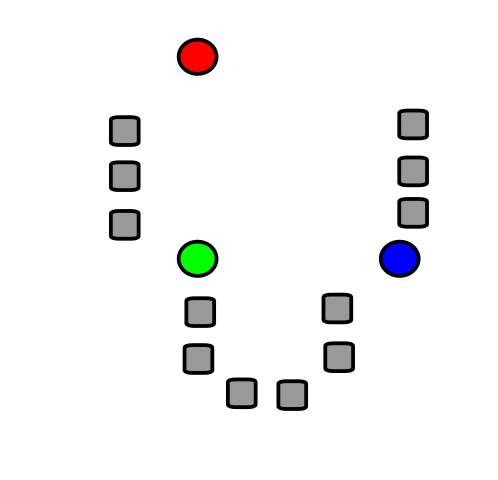
\includegraphics[width=0.95\textwidth]{kmean1.png}
        \caption{Original data}
    \end{subfigure}
    \begin{subfigure}{0.3\textwidth}
        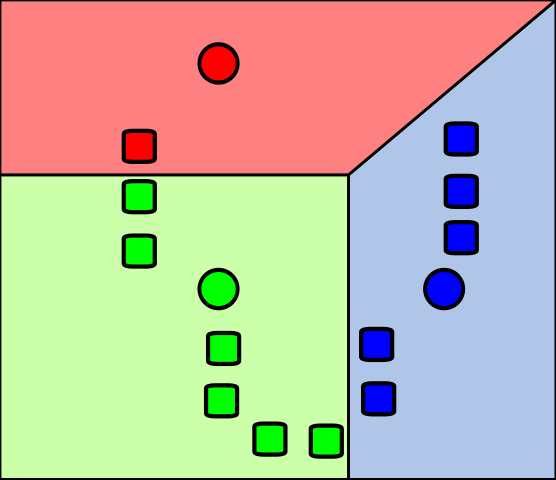
\includegraphics[width=0.95\textwidth]{kmean2.png}
        \caption{First iteration}
    \end{subfigure}
    \begin{subfigure}{0.3\textwidth}
        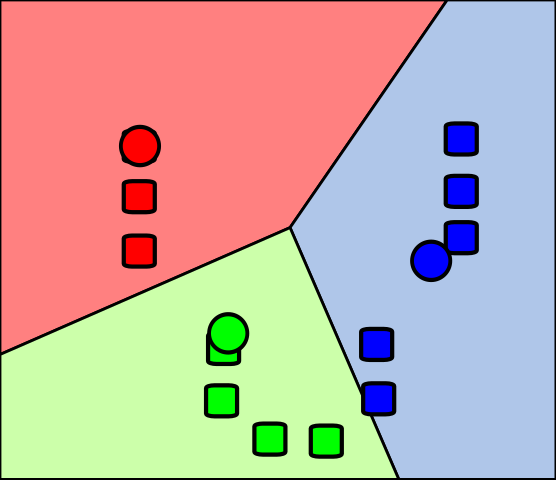
\includegraphics[width=0.95\textwidth]{kmean3.png}
        \caption{Second iteration}
    \end{subfigure}
    \caption{A demonstration of K-means clustering with three centroids \cite{kmeanspic}.}
    \label{fig:kmeans}
\end{figure}

\begin{figure}
    \centering
    \begin{subfigure}{0.3\textwidth}
        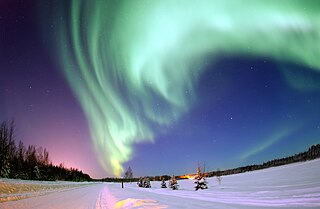
\includegraphics[width=0.95\textwidth]{kmeansreal1.jpg}
        \caption{Original image}
    \end{subfigure}
    \begin{subfigure}{0.3\textwidth}
        
\includegraphics[width=0.95\textwidth]{kmeansreal2.png}
        \caption{$k=16$}
    \end{subfigure}
    \begin{subfigure}{0.3\textwidth}
        
\includegraphics[width=0.95\textwidth]{kmeansreal3.png}
        \caption{$k=2$}
    \end{subfigure}
    \caption{Segmentation of a digital image. \cite{kmeanspicreal}.}
    \label{fig:kmeansreal}
\end{figure}


Methods like k-means allow for the segmentation of images into 'meaningful' partitions. These clusters may correspond to useful semantics---such as the separation of colors in an image---which may be modified or analyzed independently.

\paragraph{Advanced Methods} Moving beyond simple clusters, techniques have also been developed to analyze the 'edges' of objects within an image. Using methods of \tech{edge detection}, it becomes possible to asses the physical shapes and locations of objects within image data \cite{ziou1998edge}. This is done by considering the 'rate of change' of data within an image. For example, consider a black-box framed as the center of an (otherwise white) image. The pixel value at the edge of the box would be something like:

$$f(x_{e}, y_{e}) = 0$$ 

But the pixels surrounding it---the white which lies outside the box---instead have the values:

$$
f(x_e + 1, y_e + 1) = 255
$$

This sudden shift in value is detectable using methods rooted in calculus such as \tech{image derivatives.} \cite{hashimoto1987multiple}. Although the specific mathematics driving edge detection are outside the scope of this paper, we must take a moment to talk about a relative field of study---\tech{corner detection}. 

As one may guess from its naming, corner detections runs parallel to edge detection---working to assess the corners of objects within an image instead of entire edges. Similar (in abstract) to edge detection, corner detection calculates edges using image derivatives---with the additional requirement of large shifts in both the $x$ and $y$ directions of an edge. Or, to use the formal phrasing, corners are points with a low \emph{'self-similarity. \cite{maver2009self}'} Methods of corner detection were popularized by Harris and Stephens in 1988, as we will see in later chapters \cite{Harris}. 

\subsubsection{The Diffusion of Computer Vision}

Using these methods (and many others left unexplored in the interest of brevity), the act of analyzing a digital image---particularly for its regions of interest---becomes possible. Contemporary open source libraries such as \tech{OpenCV} \cite{opencv_library} have accelerated the spread of computer vision techniques by providing an extensive and high quality collection many classic computer vision algorithms. We will continue to review computer vision topics in later chapters. For now, we turn to AI and machine learning. 

\subsection{AI \& Machine Learning}
It is clear that providing even a brief overview of AI literature is beyond our scope. Consequently, we will be focusing on topics of relevance in the fields of machine learning.

\subsubsection{Machine Learning: A Brief Review}
Machine learning (\tech{ML}) is, in its essence, the marriage of statistical modeling techniques and computer technology \cite{mahesh2020machine}. ML centers around the development of \tech{models} which serve to predict an output based on a particular input. More specifically, the goal of a model---once completed---is to predict output \emph{without} the helping hand of its creator. 

This requires the model to be \emph{'trained'} with a series of known inputs and outputs. When first constructed, the model is essentially a collection of random functions---turning any given input into functionally random output. As training data inputs are fed into the model, each (again, initially \emph{random}) output is compared against the known 'correct' outputs found in the training data. The inner-workings of the model's functions are then slightly adjusted based on the model's output prediction error \cite{jordan2015machine}. 

Generally---given enough statistically significant training data---a model may eventually become 'trained.' This trained model is capable of taking any given input and producing a good approximation of output. This is because the internal functions of the model---which once spewed random noise---were slowly 'shaped' over time (via the training data) into functions that actually fit the nature of the model's question \cite{mahesh2020machine}. 

\paragraph{Neural Networks }

Many machine learning paradigms extend this simple concept with additional theories and stipulations. Most notable is the model of a \tech{neural network}\footnote{Also referred to as an \tech{Artificial Neural Network} (\tech{ANN}) \footnote{abiodun2018state}} and its extensions \tech{deep learning} and \tech{reinforcement learning.} Neural networks frame the issue of machine learning in terms of the biological neural networks found in animal brains. Each input \tech{neuron} makes connections to other neurons, eventually reaching a series of output neurons. The connections between neurons are the model functions described above. Neurons are traditionally grouped into several \tech{layers}: the \tech{input} and \tech{output} layers, as well as any number of \tech{hidden} layers which lie between the two. The name stems from its vague similarities to brain structure---each neuron forming convoluted connections to all of the neurons in surrounding layers \cite{dongare2012introduction}.

\subparagraph{Deep Learning} 

A neural network is said to feature deep learning when using many neuron layers, as well as a wealth of training data. This is because the 'deep' nature of deep learning models' neuron structures are capable of learning things 'deeply.' Or, in other words, capable of learning 'representations of data with multiple levels of abstraction \cite{lecun2015deep}.' The model's ability to predict several layers of semantic nuance has made them a good fit for multi-modal and multi-contextual tasks such as image and text classification \cite{minaee2021deep}.

\subparagraph{Reinforcement Learning}

Reinforcement Learning, meanwhile, bucks the trend of training data altogether. Instead of providing static, prepared training data, reinforcement learning models provide \tech{reward} metrics. When a model makes an output prediction, its accuracy is evaluated and a proportional reward signal is sent to the model. The model then adjusts its internal functions based on the reward signal---constantly attempting to maximize received rewards \cite{kaelbling1996reinforcement}.   The \tech{NEAT} (\textbf{N}euro\textbf{E}volution of  \textbf{A}ugmenting \textbf{T}opologies) method \cite{NEAT} is one notable implementation.


\paragraph{MarI/O}

We will now review a simple example to reinforce our learning. Injecting some levity and topicality into our discussion, we consider a machine learning model trained to play the ever-popular \emph{Super Mario World.} In 2015 \emph{SethBling\footnote{A noted online personality in the realm of games and computer science. Real name Seth Hendrickson.}} demonstrated a machine learning model that successfully played \emph{Super Mario World} \cite{sethbling} in a video viewed by over 11 million people, garnering significant press coverage \cite{Souppouris_2015} \cite{Gallagher_2015}. Hendrickson's model---named \tech{MarI/O}\footnote{Source code available at \cite{Hendrickson_2015}.}---is based on the NEAT method discussed above.


What constitutes 'input,' 'output,' and 'reward' naturally differs significantly depending on the model. In the case of MarI/O, the model receives a simplified representation of the game-world (designed by Hendrickson) as input and produces a in-game command as output. The model's input consists of key data such as the location of Mario, enemies, and items, while the output is a simple button press on a controller such as \tech{UP} or \tech{A.} The reward function used for reinforcement is based on how far Mario progresses within the given level. This is an incredibly simple metric to measure---as most \emph{Super Mario World} stages move purely left-to-right. In other words, the further Mario 'moves to the right' within a level, the more rewarded the model is. 

Hendrickson allowed the model to train for 24. To improve training efficiency, he forced a level reset if Mario failed to move within a given time window. At first, the model produced only poor results---often remaining motionless. Eventually, the model randomly produced a \tech{RIGHT} output, which moved Mario forward. This decision received a large reward, altering the model's internal functions in ways that biased it to continue outputting \tech{RIGHT} commands. Although a successful start, the model failed whenever Mario reached obstructing objects. Eventually, a random combination of \tech{RIGHT} directional inputs and \tech{A} button presses allowed Mario to progress further in the level---giving the model additional rewards and further altering its internal functions. 

We can now see how MARI/O achieved mastery of its task---by producing random outputs until the outputs are deemed successful, which alters the model's behavior. With enough iterations (and using reasonably valid assumptions), it becomes possible to train a litany of models to produce good output estimations over an even wider array of problem domains.  

\subsubsection{Object Recognition and Classification}
Most crucial for our research are the advances made in \tech{object recognition} and \tech{object classification}. One may imagine how the research discussed above empowers these tasks. Recognition models are usually trained on massive data sets featuring thousands of images. These images are \tech{annotated} with \tech{features} that the model is trained to recognize \cite{wang2016deep}. For example, a face detection model would likely train on images featuring human faces. Each face is manually labeled and perhaps includes  other key characteristics (age, gender, race, etc.) used in training and tuning the model. A small sub-set of training data is usually unused in training, instead being set aside to 'test' the model's post-training validity. The trained model is considered valid if it produces output matching known 'correct' output in the testing data \cite{zhao2019objectdetectiondeeplearning}. 

We will explore these topics further in the following chapters. For now we turn our attention to other fields of relevant research. 

\section{Spatial Audio}
In this section we explore theory and research related to \tech{auditory displays}---from \tech{audification} and \tech{sonification} to \tech{spatial audio} and \tech{3D Audio}.

\subsubsection{Auditory Displays, Audification, and Sonification}
Our work deals with \tech{auditory displays}---systems which employ "the use of sound to communicate information about the state of a computing device to a user \cite{audiodisplays}." More specifically, we utilize \tech{sonification} techniques. Sonification was defined by Scaletti as "a mapping of numerically represented relations in some domain under study to relations in an acoustic domain for the purposes of interpreting, understanding, or communicating relations in the domain under study \cite{kramer1994auditory}." In simpler terms, sonification is the translation of information from other domains into audio\footnote{We should note that the definitions of audification and sonification are somewhat vague in the literature. As seen in \cite{vickers2017directsegmentedsonificationcharacteristic}, audification is sometimes considered a subset of sonification---one that deals with the \emph{direct} one-to-one translation of non-audio data into audio data. However, as these terms maintain some flexibility, we have opted to use 'audification' in our research.}. Sonification is a complex research field that combines "psychological research in perception and cognition" with the development of computer "tools" and software "design \cite{kramer2010sonification}." Many core research topics overlap with physiology, psychology, acoustics, cognition, signal processing, and computer science. 

We will now review a few concepts from the field relevant to our research.

\subsubsection{Sound Localization}
Most key to our research is the topic of \tech{sound localization}. Humans, along with numerous animals, are capable of localizing the origin of sounds in three dimensions \cite{middlebrooks2015sound}. \tech{Interaural time-difference cues} (\tech{ITDs})---the difference between a sound signal as it reaches each ear indecently---was devised as a model for understanding sound localization. Lord Rayleigh proposed theories of sound localization in horizontal planes termed \tech{duplex theory}, which ITDs model. In essence, it is observable that the difference in \emph{travel-time} (i.e., path length) between a sound's origin point and each of the listener's ears produces a distinct localization of the sound in the human mind \cite{middlebrooks2015sound}. ITDs were later modeled by Woodworth mathematically:

$$
ITD = \frac{a}{c}[\theta_{rad} + sin(\theta_{rad})]
$$

Where $a$ is the radius of the relevant sphere (i.e., the human head), $c$ is the speed of sound, and $\theta$ being the angle of the sound relative to the listener \cite{woodworth1954experimental}.

\subsubsection{The Head-Related Transfer Function}

As one may imagine, the specific characteristics of localization depend on the physiology of the listener. Not all heads and ears are made alike, after all. The \tech{Head-related transfer function} (\tech{HRTF}) models this behavior \cite{li2020measurement}. The specific derivations of an HRTF are beyond the scope of this thesis, but we must note a few key observations. A high-quality HRTF is required for good spatial audio reproduction. However, a challenge lies in the fact that HRTFs are unique to the individual---and must be calculated per-person if precise results are desired. Consequently, spatial audio technologies supply 'average-case' HRTFs, which are sufficiently effective in general situations. HRTFs also presume an 'open-field' (that is, a room without any acoustic characteristics), meaning that additional acoustic information must be provided after-the-fact \cite{moller1995head}. 

\subsubsection{Spatial Audio and the 3D Audio Effect}
Recent advances in spatial audio technology have married these two details---precise, research derived HRTFs, and \textbf{room modeling} (the simulation of acoustics) \cite{roommodel}---to great success. As we described above, humans localize sound in \emph{three} dimensions---meaning \tech{hight channels} are necessary to accurately produce a \tech{3D audio} effect. We are, of course, referring to the \tech{channels} used in modeling \tech{surround sound} technology---the more common \tech{center} and \tech{surround} channels are also needed to produce 3D audio \cite{3daudio}. 

Contemporary research from laboratories such as Dolby have produced technologies such as \tech{Dolby Atmos}, which incorporates hight channels, room (i.e., acoustic) metadata, and a conceptualization of \tech{audio objects} to ease the generation of 3D audio \cite{Pfanzagl-Cardone2023}. Non-surround sound technology also makes use of Atmos and similar 3D audio branding. To achieve a similar effect, HRTFs are used to estimate and exaggerate spatiality, combined with room metadata and audio objects \cite{dewey2024practitioners}.  

Many advances in modern spatial audio originate from games-adjacent research, which we will cover in the next section. 

\section{Games}
We at last arrive at the core field of our research---games. We shall begin with a review of relevant accessibility research before considering similar work in the realm of audification and computer vision before finally concluding this chapter. 

\subsection{Games and Accessibility}
As described in the previous chapter, there has been an increasing trend towards accessibility in the games industry. One industry survey---commissioned by the causal game company \emph{PopCap}---found that over 20\% of their userbase identified as disabled \cite{Popcap_2008}. Similar examinations have shown games to be a popular pastime for disabled persons, despite high barriers of entry---especially in action-focused genres \cite{yuan2011game}. The trend eventually received headline attention in 2015 when the United States of America's Federal Communications Commission imposed legal requirements for improved accessibility on the gaming industry \cite{Richert}.

Naturally, there has also been a growing body of research on games and accessibility. Previous work has laid the groundwork motivations for game accessibility research \cite{miesenberger2008more} \cite{garber2013game} and critically examined barriers to widespread adoption \cite{porter2013empirical}. Others have sought design of bespoke accessible games \cite{AudioArchery}, while many more have proposed bespoke after-market modifications of existing games \cite{atkinson2006making}. Others still have performed comprehensive surveys of accessibility features in popular titles as well as user impressions of these features---identifying middleware as a 'critical link' in the 'chain of accessibility \cite{porter2013empirical}.'

\subsubsection{Defining Games Accessibility}
Previous work has endeavored to formally define and categorize games accessibility concepts. \cite{yuan2011game} partitioned target demographics into those with \tech{vision, hearing, motor,} and \tech{cognitive impariments}---based on WHO guidelines in \cite{world1980international} as well as \cite{accessguidelines}. The authors then proceed analyze the accessibility and the gaming experience through the lens of gameplay loop made of three phases---\tech{receiving stimuli}, \tech{determining response}, and \tech{providing input}. They then consider challenges and solutions for improving this loop for each disability category. Speaking on the visually impaired, the authors conclude that even though these players are "physically able to perform" gameplay tasks, they are "unable to perceive primary stimuli" and that "without this feedback, it is impossible to determine what in-game responses and what physical input to provide \cite{yuan2011game}." 

Echoing general consensus the authors in \cite{yuan2011game} later conclude that good accessibility features for the visually impaired should replace visuals with audio---providing audio cues and sonification to inform players on otherwise absent primary stimuli.

\subsection{Games and Audification}
Despite this, the authors in \cite{prazaru2020overview} observe cases where visually impaired users claim mastery over games not designed specifically for their impairments---such as in \emph{Mortal Kombat}. This is (in some part) due to the neurological theory of \tech{brain plasticity}---a phenomenon wherein un-used parts of the brain (e.g., visual processing centers) are reused for other tasks \cite{nudo2006plasticity}, thereby affording visually impaired users additional 'brain capacity' for processing audio information. They explain that \emph{Mortal Kombat} in particular is accessible (albeit unintentionally) to visually impaired users on account of its wide array of distinct and heavily signaled audio cues for different character moves and attacks. In general, repeated research has shown that improved auditory feedback 'helps visually impaired individuals move faster in a game \cite{agrimi2024game}.'

\subsubsection{Audio Games}

This is reflected in the wealth of existing \tech{audio games}, which either supplement or entirely replace the visual component of games with audio-oriented techniques. Or, to use the phrasing found on \texttt{audiogames.net}---the largest repository for audio games online: 

\begin{quote}
\emph{"An audio game is a game that consists (only) of sound. Its gamemechanics [\tech{sic}] are usually based on the possibilites [\tech{sic}] of sound as well. Usually (but not always) audio games have only auditory (so no visual!) output. Audio games are NOT specifically games for the blind! It is true that most audio games around at the moment are developed by and for the blind community. But we think audio games have the potentional [\tech{sic}] to be a genre on its own due to the immense undiscovered possibilities of sound. We believe that audio games have the potentional [\tech{sic}] to be a complete gaming genre on its own."} \cite{Audiogames}    
\end{quote}




The authors of \cite{friberg2004audio} analyzed the trend of audio games, proposing a semiotic model of sound in games that considered gaming through the \tech{casual, semantic,} and \tech{reduced} listening modes. They also make inroads at merging theory with practice by demonstrating the \tech{TiM} (\tech{T}actile \tech{I}nteractive \tech{Multimedia}) project, a development of the Stockholm International Toy Research Center. The TiM project evaluated the efficacy and possibilities of audio games through three self-made titles: \emph{Mudsplat}, \emph{X-tune}, and \emph{Tim's Journey}. Through their work, they demonstrate 'functional' design solutions that prove even visually impaired children are capable of handling complex control interfaces. Moreover, the authors proceed to argue that 'sound-based games' do not have to be developed only for players with visual impairments. 


The authors of \cite{urbanek2019unpacking} ventured to gain an 'in-depth understanding of the audio game experience.' They also surveyed tools for creating audio games---finding a dearth of information. They go as far as stating that they could find "(almost) no documentation or reflection of the processes that [other] researchers engaged in when designing their games"---highlighting a need for more audio game development tools.

Despite this, some have managed bespoke development of audio games. The first noteworthy example is Japanese game director Kenji Eno's \emph{Real Sound: Kaze No Regret}\footnote{Originally released exclusively in Japan for the Sega Saturn in 1997. The game has since been re-released in audio drama format.}, which is (to this author's knowledge) the only audio game ever brought to mass-market. According to Eno, the game was inspired by letters he had received from blind fans following the success of his 1995 horror game \emph{D}---which featured a slow paced, atmospheric, and puzzle-oriented design attracted blind players by chance \cite{Torres_2005}. The game was a modest success, being re-released on the Dreamcast in 1999.

While \emph{Real Sound} may be the only mass-market audio game, there have also been many other notable entires in the medium. The enduring popularly and open-source nature of id software's \emph{Doom} and \emph{Quake} series have naturally extended themselves to the audio game community as well. \emph{Shades of Doom} \cite{GMA_Games} and \emph{AudioQuake} \cite{atkinson2006making} are two such examples, which modify each game's source code to include audification features and other accessibility support. AudioQuake has since expanded into the \tech{AGRIP} project, including support for custom level designs via its 'level description language \cite{Atkinson2009}.'


Others have sought ground-up re-creations of iconic titles---such as \emph{Mach 1 Car Racing}---a remake of Namco's arcade classic \emph{Pole Position} \cite{friberg2004audio}. There has also been a successful niche of audio rhythm games---such as \emph{Blind Hero} \cite{yuan2008blind}, \emph{Finger Dance} \cite{miller2007finger}, and even \emph{Metris} \cite{metris}, a musical version of \emph{Tetris}. The recent indie game \emph{Blind Drive} \cite{blinddrive}, was developed from the ground up as a commercial release and brought audio games to entirely new audience outside of research circles.

\subsection{Games and Computer Vision}
Recent years have also seen a growing interest in the intersection of games and computer vision. 

One common application has actually been the usage of computer games to train computer vision models---as games are able to produce easily understandable and realistic data on-the-fly \cite{shafaei2016play} \cite{richter2016playing}. Others have considered ways to integrate computer vision into development processes---\cite{qiu2016unrealcv} merged openCV with the Unreal engine while \cite{paduraru2021automated} proposed methods of automating game testing through CV methods.

There has been some overlap between computer vision, games, and accessibility (and serious games) research. The authors of \cite{chursin2021using} proposed an educational game making use of computer vision, while \cite{webgame} demonstrated an online game used in training a computer vision model that improves website accessibility.

\subsection{Related Work}

Lastly, we note a few research efforts bearing resemblance to our own work. \cite{erdelyi2019using} performed similar research by using computer vision techniques and a bespoke algorithm to achieve computer-automated gaming. \cite{vallejo2011applying} also produced a similar result to our own proposal---integrating audification tools (sans computer vision techniques) into a custom point-and-click adventure game engine. The very recent work of \cite{StreetFighter}, meanwhile, examines the implementation of audification techniques in the newly released hit fighting game \emph{Street Fighter 6}, which received new accessibility features around the time of writing. 

\subsection{Conclusion}
In this chapter, we reviewed theories and research relevant to our proposal. We began with an overview of computer vision research---namely in the areas of image processing and analysis---before moving onwards to AI and machine learning research. There, presented a brief summary of machine learning topics and considered an example using video games. We also made a brief stop to review the fields of object recognition and classification.  

Afterwards, we switched disciplines and reviewed spatial audio theory---staring with concepts of sound localization before transitioning to discussions on spatial audio and 3D audio effects. 

Finally, we turned our focus to games---beginning with a look at games accessibility research. We then mediated on audification research as it related to games---particularly through the lens of audio games. Then, we took a look at the intersection between computer vision and games research before finally making brief considerations of work similar to our \rs proposal.

Although this chapter forms an adequate summary of relevant topics, we will continue to introduce and review theory as needed in the following chapters as well. We now move to a detailed proposal and exploration of the \rs system.


%%% PROPOSAL

\chapter{ReAL Sound}
\paragraph{Introduction}
In this chapter, I propose and outline the \textbf{\emph{\rs}} system: a \rsfull that abstracts the design of accessibility features for the visually impaired via the use of computer vision, spatial audio, and audification techniques.

\section{Proposal} 
\paragraph{Introduction} 

In this section, I propose \rs and justify its novelty and utility based on the literature review performed in the previous chapter.

\subsubsection{\emph{What is \rs?}}
\rs (\rsfull) is a software framework concept that generalizes the creation of visual accessibility features for games. Using computer vision techniques and modern spatial audio technology, \rs aims to abstract the process of moment-to-moment analysis of a game's state as well as the generation of 3D spatial audio objects. Through this abstraction, implementors of \rs (as distinguished from \emph{users} of \rs---the visually impaired persons benefitting from the features) can sidestep many of the language, platform, and architecture specific headaches involved in the creation of game accessibility features, especially in the case of after-market games. 

In essence, \rs seeks to convert a game's visual information (the things a player sees on-screen) into audio information (the things a player hears). This is done so that visually impaired persons can better understand a game without having to 'look' at it directly. Moreover, \rs aims to abstract this process, making a simple implementation possible for a plethora of games. \rs achieves this generalization by abstracting feature development process into a few core steps for any given target game:

\begin{description}
    \item [Planning] The creation of simple 'rules' and 'definitions' which accurately describe the game.
    \item [Training] The act of preparing computer vision techniques based on the \textbf{Planning} stage to analyze the game's current state data.
    \item [Design] The creation of simple 'rules' and 'definitions' for translating the data analyzed in the \textbf{Training} phase into spatial audio objects. 
    \item [Execution] The real-time marriage of the previous stages. Uses a computer vision model \textbf{trained} on the \textbf{planned} rules which translates the game's real-time visual data into spatial audio objects as \textbf{designed} by the implementor.    
\end{description}

With \rs, a implementor with only a moderate amount of technical knowledge  could feasibly add accessibility features to any target game---all with zero knowledge of the game's underlying source code or architecture. A visually impaired user of \rs, meanwhile, gains access to accessibility features which translate the game's visual information into easily parsable audio data---allowing them to intuitively understand a game without seeing the game's visual output. 


\subsubsection{\emph{Why is \rs?}}
As discussed in the previous chapter, there is a well-established and ever-growing need for software interoperability and platform agnostic support, as well as a growing demand for improved software accessibility. Implementors of game accessibility features already face numerous game-specific challenges in the design process---as each game's bespoke nature demands equally unique accessibility design. The added barriers of specific architecture, engine, and language implementation have especially stymied the development of accessibility features in the gaming industry---where many development tools target a single architecture or operating system, are company specific, and are often used on a per-game basis. 

\rs significantly streamlines these problems through abstraction---significantly simplifying this troubled implementation process. As a consequence, greater flexibility and more time are handed to feature designers---who are now better quipped to craft higher quality features at a faster clip.

Moreover, the generalization process requires zero knowledge of the game's actual codebase, meaning games can be modified in the after-market by dedicated enthusiasts. As a consequence, the fan-driven movement of retrofitting of older titles with modern accessibility features becomes easier---allowing visually impaired persons access to a wealth of classic titles while costing modern developers zero resources. This is becoming especially crucial in modern times, as some estimates show that over 85\% of games are functionally abandoned---with no publisher or developer entity maintaining ownership \cite{Lewin_2023}. This fact effectively renders the vast majority of published games, \emph{'abandonware'} with little hope of official improvements by original developers \cite{Costikyan_2000}.

\subsubsection{\emph{How is \rs?}}
\rs is made possible through modern machine learning, computer vision, and spatial audio technologies. Using the latest computer vision techniques through libraries like OpenCV\cite{opencv_library}, even novice developers can implement object detection algorithms---which analyze visual input and return semantic information about the its contents---with ease. 

\paragraph{The Modern AI Boom}

On top of this, the recent 'boom' in AI technologies\cite{Knight_2023}\cite{Meredith_2023} has brought an equally intense focus to the development, improvement, and democratization of AI tools and systems\cite{Brynjolfsson_McAfee_2017}\cite{Heikkilä_2022}. Ecosystems like \emph{HuggingFace}\cite{Wiggers_2022} and projects like Google's \emph{TensorFlow}\cite{tensorflow2015-whitepaper} have dramatically changed the landscape of AI technology development---trivializing many tasks considered inaccessible to the common developer just a few years ago.

\subparagraph{Agnostic Vision Requirements}

Considering the ever-changing state of modern AI and computer vision technology, \rs does not specifically call for any one particular solution for its \textbf{Training} or \textbf{Execution} stages. Instead, \rs only requires the \emph{successful} real-time identification of in-game objects \textit{as defined by the implementor}. The means by which this goal is accomplished is left up to the implementor, and may be achieved by any available means. 

Consequently, \rs does not technically demand the usage of AI \emph{at all.} Many well-proven pre-AI techniques---such as \emph{template matching}\cite{Brunelli2009-gh} and \emph{corner detection}\cite{Hildreth1980}---have proven to be successful in many simple use-cases. I will demonstrate this in a later chapter, creating one  implementation of \rs using the original corner detection algorithm---the \emph{Harris corner detector}\cite{Harris}, originally developed in 1986. 

\paragraph{Spatial Audio}
Running alongside the AI boom has been a comparably smaller (yet not insignificant) boom of 3D and spatial audio technologies. As discussed in the previous chapter, many advances have been made in sonification, audification, and spatial audio techniques in recent years. This trend has given end-users an abundance of choice for low-cost, high quality audio playback devices with native spatial audio support--from in-ear monitors like the the Apple \emph{AirPods}\cite{ApplePods} to even computer display monitors from major manufacturers like Dell\cite{Campbell_2025}. Future patents promise even greater advancements through advanced techniques like automatic HRTF adjustments specific to the user's unique physiology\cite{Antti2024}.


Many new software development libraries been developed to address this boom in consumer demand. Fan driven efforts like the \emph{Spatial\_Audio\_Framework}\cite{McCormack2024} as well as company-produced projects such as Valve Software's Steam Audio\cite{Valve} have seen popular adoption. Legacy libraries with widespread adoption, such as the quarter-century old \emph{Qt} application development framework\cite{QTProgramming}, have also introduced support for modern spatial audio technologies in recent versions\cite{QTSpatial}. The implementations of \rs presented later in later sections utilize Qt as a backend framework---although numerous other libraries feature equivalent functionality. 

\paragraph{Conclusion}
In this section, I proposed \rs and provided justifications for its utility and novelty by considering contemporary technology innovations and emergent user trends. 





\section{Concepts}
\paragraph{Introduction} 
In this section, I explain in detail the theoretical concepts which underpin \rs. I later use these concepts to rigidly define the system's core structure. To begin, I use formal math notation to construct a semi-formal definition of a 'video game.' I then explore this definition through the lens of automata theory. Following this, I use the construct to abstract methods of interpreting a game via visual analysis. 


\subsection{Anatomy of a Game}
\subsubsection{Introduction}
Here, I construct a semi-rigid abstraction of video games using formal notation. Later, I will use these constructs to more clearly explore related concepts.


\subsubsection{Game}
A Game, termed $M$ (for \emph{meta}), can be conceived as the combination of three sets: a collection of meta attributes $A$, a series of in-game states $G$, and a group of entities $I$:

$$
M = \{A, G, I\}
$$

\paragraph{Meta Attributes}
The game's meta-attributes $M_A$ can be imagined as data that is preserved over an entire game session. This data can persist between state transitions and usually describes overarching information such as current playtime or the currently active game level. 

\subsubsection{Game State}
Each state, $G_S$ (referred to interchangeably as \textit{game state} hereafter) is comprised of four components---internal state-attributes $A$, internal state-logic $L$, as well as conditions $C$ for inter-state transitions $T$.

$$
G_S = \{ A, L, C, T \}
$$

\paragraph{State Attributes}
A state's attributes $A$ act similarly to the game's overarching meta attributes $M_A$, but on a per-state context. These attributes may store information such as the current time spent within the state or other data describing the state in specific. State data is lost upon transitioning to a different state.

\paragraph{Internal Logic}
The state's internal logic $L$ defines all the behaviors and activities that are carried out \textit{within} the state. For example, a racing game may contain a \textbf{start} state---which contains logic for playing a special sound effect when the race is started, or routines to visually display the text \textit{'START!'} on-screen. 

In abstract, $L$ can be imagined as a series of conditional requirements ('rules') $L_C$ that yield specific game actions ('responses') $L_A$:

$$L: L_C \longrightarrow L_A$$


\paragraph{Conditions}
A state also contains conditional rules defining when to exit the state and transition to different state. $C$ defines these rules as a set of boolean statements---which evaluate to either \texttt{true} or \texttt{false}.
Take, for example, a sports game which transitions from a \textbf{match} state to a \textbf{finish} state after ten points are scored in the match. Imagine that the current match score is stored as an integer value through the state attribute $S$: 

$$
S: [0, 10],  S \in G_A
$$

Then there is a condition within $C$, lets call it $C_S$, which might look like this:

$$
C_S = S\geq10 
$$

When $C_S$ evaluates to true (i.e., when the match score has reached ten points), the state will transition transition to the \textbf{finish} state.

\paragraph{Transitions}
The transition function $T$ defines the mapping of "where" to or "how" to transition to a different state after a condition in $C$ has evaluated to \texttt{true}. In essence, $T$ maps a conditional statement $C_S$ to the next game state $G_N$ to transition to:

$$
T: C_S \longrightarrow G_N
$$

This function can be generalized by instead taking a specific state $G_S$ and a generic condition $C$ as input:

$$
T: G_S \times C \longrightarrow G_N
$$

\subsubsection{Entities}
Entities $I$ are the objects which constitute a game's internal structure---the 'actors' of the game. An entity can be anything contained within a game, such as the player, enemies, items, level construction, etc.  Usually, an entity's behavior can be described using verbs---in either an active (\emph{Mario jumps on the platform}) or passive (\emph{The platform was jumped on by Mario}) sense.

Each entity has attributes $A$ as well a collection of states $E$:

$$I = \{A, E\}$$

\paragraph{Entity Attributes}
Similar to the previous definitions, entity attributes describe entity-specific attributes. For example, an entity's location point $P$ in a 2D game's world space might be modeled as:

$$P = \{(x,y): x,y \in \mathbf{R} ^2\}$$ 

Similar information, like a enemy's current health, an item's purchase price, or a bomb's damage radius are also considered Entity attributes. 

\paragraph{Entity States}
An entity state, then, describes an entity's different states of being. A player entity might be able to \textbf{jump}, while a spell entity might be \textbf{cast} or an enemy entity might be \textbf{killed}, to name a few examples. 

Some examples may seem unintuitive, but still work within this framework. A game's menu system, for instance can also be considered an entity. In this case, the act of clicking on the menu---triggering some sort of effect, can be modeled as a \textbf{clicked} state with its own internal logic and goals. 

As you might guess, a entity state looks similar to a game state, with its own internal logic $L$, a series of transition conditionals $C$, and transition mappings $T$:

$$E = \{L, C, T\}$$

One example of an entity state is \textbf{jumping}, which may transition from \textbf{idle} or \textbf{walking} or \textbf{running}. When transitioned to, the \textbf{jumping} state might, according to $L$, play a jumping sound effect. When a condition in $C$ is satisfied (the jumping entity finally touches the ground again, or perhaps falls into a pit and dies), then the transition function $T$ moves to the next state $E_N$:

$$T(C) \longrightarrow E_N$$

\subsubsection{Summary}
To summarize, a game $M$ can be conceptualized as:

\begin{enumerate}
    \item A collection of attributions ($A$), which describe aspects of the game's overarching meta-state.
    \item A set of game states ($G$), which each contain internal game-logic ($L$), state-specific attributes ($A$), as well as rules for when to transition to another state ($C$) and exactly which state to transition to ($T$).   
    \item A set of entities ($I$) which serve as the game's passive and active subjects, each having their own set of attributes ($A$) and states ($E$). Each state compasses the same qualities of a state enumerated above ($A$, $L$, $C$, and $T$).   
\end{enumerate}

$$
M = \{A, G, I\}
$$

$$
G_S = \{ A, L, C, T \}
$$

$$I = \{A, E\}$$

$$E = \{L, C, T\}$$


\subsubsection{Limitations}
While this construction is useful for our purposes here, I do not contend this definition as a end-all definition of games. It is already known that several games---both in physical and video formats---are Turing complete, which exists outside the definitions given here. Previous researchers however have likewise made attempts in formally defining games with similar bounds on their definitions---leaving titles like \emph{Magic: The Gathering}\cite{churchill2019magicgatheringturingcomplete} or \emph{Minecraft}\cite{Hildreth1980} out of scope\cite{Demaine}. Virtually any game can also be made Turning complete if methods of arbitrary code execution (ACE) are discovered, which has been demonstrated using \emph{Super Metroid}\cite{Mawhorter_Aytemiz_Karth_Smith_2021}, \emph{The Legend of Zelda: Ocarina of Time}\cite{OoT}, and numerous others. Despite this, we find that our definition of games covers a sufficiently useful scope to demonstrate \rs's utility.


\subsubsection{Conclusion}
Here, I have provided a general outline of games in formal notation. I do not guarantee nor contend that these structures form a complete closure over the entire concept of video games---whose definition is still fiercely debated to this day\cite{Knoop_2021}---but these structures will serve as a useful framework for our following definitions and concepts.

\subsection{State Models}

\subsubsection{Introduction} 
In this section, I briefly review automata theory theory. Through concepts like finite state automata, I produce the Game and Entity (GSM and ESM) state machine constructs, which I will continue to utilize in following sections.

\subsubsection{Automata Theory}
The previous section's underlying theory will likely seem familiar for those with a background in fields such at theory of computation or advanced linguistics. I am, of course, referring to the theory of \emph{automata} a core concept which underpins numerous fields--including computing and, by natural extension, interactive software such as video games. 

Automata are generally categorized into four major types as defined by the Chomsky Hierarchy---ranging from Type-0, describing the classical Turning machine, to Type-3, which describes finite state automata \cite{Chomsky1956ThreeMF}. Games, as I have described them above, can (in general) be described as a Type-3 automata---an automation of finite state and quality. 

\subsubsection{Finite State Automata}

\paragraph{Introduction and Concepts}

Carroll defines (deterministic) finite automata as the "mathematical model of a machine that accepts a particular set of words over some alphabet $\Sigma$.\cite{FSM}" He conceptualizes FSMs as "black boxes" that combine an input tape (consisting of symbols in the alpha $\Sigma$), a \emph{'read head'} which processes this input tape of symbols, and an 'acceptance light' which indicates the acceptance/rejection of an input symbol, and whose activity is governed by the read head's reaction to the given input. In essence, the machine accepts input, makes decisions for the acceptance light based upon the input, and then moves to a new position to receive another input. The machine's acceptance/rejection of a symbol, as well as the position it moves to next, is contingent on its own internal logic---some rule that dictates \emph{"If symbol X is read, turn on (if accepted) or off (if rejected) the acceptance light, and move read head to position Y."} The machine may also read a symbol which finally halts its operation.

\paragraph{Comparison with Turing Machines}

This conceptual structure bares some resemblance to a Turning machine\cite{Turing}, although there are some distinct differences. A Turning machine has an infinite amount of memory and is capable of accepting languages with recursive qualities---as the turing machine is able to 'write' to tape--modifying a symbol after reading it. A Turing machine is well known to be capable of implementing and computing any possible computing algorithm\cite{Turing_2004}. It is consequently classified as a Type-0 (also known as a "recursively enumerable" or an "unrestricted") grammar.

An FSM, by contrast, is limited in several ways. As the name implies, FSM have a \emph{finite} set of states. More importantly, the system is incapable of storing memory---lacking the 'writing' mechanism of a Turning machine\cite{FSM}. 

\paragraph{Deterministic and Non-deterministic FSAs}

The FSMs we detail here should also be distinguished as \emph{deterministic}, as opposed to \emph{non-deterministic} FSMs. Some FSMs are considered non-deterministic when their states are capable of transitioning to several possible outputs given the \emph{same input}---making their reaction to an input non-deterministic in nature\cite{NDFSA}. For our purposes, we define games as a type of deterministic FSM--where the same inputs always yield the same results. 

\paragraph{Obstacles and Limitations}
You may be wondering how the provided definition of games fit the category of FSM considering the inclusion of attributes $A$---which may persist as a game or entity transitions from state-to-state. This may appear like a kind of 'memory' on first glance, but is actually just a shorthand notation that simplifies our FSM conceptualization. In reality the proper FSM of a game has \emph{many} more states than we describe here. 

To provide some insight into this concept, imagine that for each state $G_S$, the conditions of $C$ and the transitional rules of $T$ also encode the attributes of $A$. This means that each state $G_S$ actually has numerous variations---each relating to the specific attributes of $A$ and the conditions of $C$. For example, the aforementioned sport game's \state{match} state may really have $10$ different \state{match} states, one describing each possible value of the scoring attribute $S$. If the game has just begun, the first scoring condition $C_0$ will transition the machine to $match_1$, and so on. Eventually, the final \state{match} state's $C_9$ condition will transition the FSM to the \state{finish} state.


\paragraph{Useful Adaptions}

As you can see, this more-accurate representation of FSMs is considered unproductive in many domains where FSMs remain useful concepts\cite{state}. Thankfully, numerous alternative notations have arisen to address these shortcomings. 

For example, FSMs which produce output contingent on a given input---often termed \emph{transducers}\cite{FSM}---are frequently conceptualized as \emph{Mealy machines}. The output of a Mealy machine state is also contingent on its input (\texttt{IF input(X) AND IN state(Y) THEN transition(Z)}). Later designs---such as the \emph{unified modeling language}---have extended this notation further to leverage the theoretical benefits of FSAs while avoiding their limiting notation schemes\cite{omg2011umls}. In a similar fashion, I make use of FSAs on a conceptual basis while abstracting away these notational hindrances through the usage of the attributes $A$ of each object. 

\subsubsection{Automata and Games}
It is possible to define games more clearly through their relation to FSAs using our definitions. For example we can consider a game to be a collection of two principal state machines: 
\begin{description}
    \item[Game State Machine (GSM)] The game state machine comprises the general 'flow' of a game---its levels, combat encounters, win conditions, story sequences, game-over menus, boss fights, item inventories, and any other 'macro' loop that is reasonably distinguishable within the gaming experience.
    \item[Entity State Machine (ESM)] An entity state machine comprises the general 'life' and 'activities' of a given entity---every action it can take, as well as its response to any given input. A player may run, jump, or die, while a stage platform may move or vanish.     
\end{description}

These two concepts---the GSM and ESM---prove to be crucial in the conceptualization of \rs. We will continue to analyze them in later sections using other frames of analysis.

\subsubsection{Conclusion}
In this section I reviewed numerous aspects of automata theory---namely finite state automata---in order to present the concept of the Game and Entity state machines (GSM and ESM), which will prove to be useful constructs in the total construction of \rs.


\subsection{How Players Understand Games}

\subsubsection{Introduction}
In this section, I explore how games are conceived from the player's perspective. I illustrate my points via a few examples and ultimately generate the concept of the \state{State-Rule} relationship, which has consequences for \rs's design.
 
\subsubsection{How Players Understand Games}

\paragraph{Introduction}

Drifting slightly from the previous formal definitions, let us consider here exactly how a human player understands a game. To begin, let us consider a simple game familiar to most readers---the playground classic \emph{rock-paper-scissors}. 

\subparagraph{Simple Case: \emph{Rock-Paper-Scissors}}

In rock-paper-scissors, each player is allowed one input---the 'hand' they choose to play---and the game produces one 'output'---the outcome of the match. Experienced players have an intuitive understanding of the rules which govern the game, which are simple enough to enumerate here:

\begin{description}
    \item [Rule One:] Each Player produces a hand symbol, which may be one of:
        \begin{enumerate}
            \item \state{Rock}
            \item \state{Paper}
            \item \state{Scissors}
        \end{enumerate}
    \item [Rule Two:] The outcome of the match is decided by these stipulations:
        \begin{enumerate}
            \item \state{Paper} 'beats' \state{Rock}
            \item \state{Rock} 'beats' \state{Scissors}
            \item \state{Scissors} 'beats' \state{Paper}
            \item If both players produce the same hand, the game is a draw
        \end{enumerate}
\end{description}

These rules comprise the entire experience, allowing a full play of the game to occur over the course of mere moments.

To use the constructs defined previously, it is clear that rock-paper-scissors (hereafter \emph{RPS}) has only one possible game state, a fact which highlights the game's simplicity. In other words, players require no greater sense of \emph{context} to play RPS---they only need to understand the base rules described above. Consequently, the game has no memory requirements, as each play is decided in one step and has no consequences on future or past matches.

\subparagraph{Average Case: \emph{Rock-Paper-Subsequent}}
The previous definition of RPS can seem trivial, leading to an unfulfilling experience for gamers. As you likely know, many performances of RPS actually append on additional rules to improve the play experience. For example, competitions often involve some \emph{'best-of'} requirement---stipulating that a player must win a certain amount of matches before being declared the 'overall' winner. 

This example of RPS, which I will term \emph{Rock-Paper-Subsequent}, has added additional complexity to the game's structure. The logic of each round is now contingent on the last, requiring players use a sense of context and memory to successfully complete the game. For example, forgetful players competing in a 'best-of-one-thousand' variant of RPS may eventually lose-track of the game's score. This mistake would render the entire competition invalid, as it makes the question of who will win the match undecidable. 

In automata terms, \emph{Subsequent} has gained a sense of state---one for each possible configuration of game score. This case can be described in terms of an FSA, and, I conjecture, is categorically equivalent to my definition of games above.

\subparagraph{Advanced Case: \emph{Rock-Paper-Scheherazade}}
Imagine now that instead of having one simple match or even a simple 'best-of', we created a new version of RPS named \emph{Rock-Paper-Scheherazade}. In this version of the game, a tied match (where players produce the same hand) requires that players perform a 'best-of-three' sub-match of the game. Whichever player wins this sub-match will 'win' the match. This logic also applies recursively, meaning that players who tie during a sub-match are forced to perform yet another sub-match \emph{within} the sub-match---a sub-sub-match, if you will. This logic can naturally extend to an infinite recursion of context and memory: \emph{sub-sub-sub-sub-sub...-matches} are possible in \emph{Scheherazade}, each requiring the player to keep track of the game's current 'match', as well as all of the matches that exist 'above' it.

This rendition of RPS is, in some senses, comparable to a Turing machine---allowing for infinite memory and recursive processes---which extends beyond the definition of games we contend with in this paper. In this case, RPS may have an infinite amount of game states---each contextualized by the particular score of the current sub-match as well as all of the sub-matches that exist in the levels above it. 

The purpose of these examples was to illustrate in clear terms the two key parts of a game's structure from the player's perspective---\state{Rules}, and \state{States}.

\paragraph{Rules}

Rules constitute the bulk of a player's understanding of a game. Without rules, even simple titles like RPS are rendered non-deterministic---as an infinite amount of hands outside of \state{Rock}, \state{Paper}, and \state{Scissors} may be produced, each with arbitrary rules about which hand 'beats' which, which may also change on a match-to-match basis. In general, players expect a specific reaction to a given input. 

It should be noted that this is true even in cases where the output is seemingly random to the player. For example, a player always expects to be dealt a set of playing cards when performing an ante in Poker, even if those cards are given to the player in a seemingly random sequence. The player is not, by contrast, expecting to receive a collection of random objects that \emph{differ} each ante in lieu of playing cards---a gun for one hand, a hot-dog for the next, and perhaps the entirety Shakespeare's \emph{Hamlet} the last. 

\paragraph{States}

Despite this, rules are not the end-all-be-all of understanding most games---which are usually comprised of many different states. In these cases, the rules of the game actually best described as the \emph{rules of the state.} This means that the same rule, applied in different states---may actually produce a different output given the same input. This provides rules with a greater sense of context that games often demand. 

\paragraph{The State-Rule Relationship}

Consequently, one may imagine the intertwining of these two concepts: \state{Rules} which define \state{State}, and \state{States} which identify \state{Rules}. This \state{State-Rule} relationship often relates to problems in \emph{context sensitivity}, a domain which extends far beyond the realm of video games. Understanding this relationship, as well as context sensitivity, is key to \rs' design. We will now explore the problem further through a well known example: \emph{The Legend of Zelda: Ocarina of Time}, which pioneered advanced solutions to context-sensitive game design.

\subparagraph{Context Sensitivity and \emph{Ocarina of Time}}

As three-dimensional games saw increasing feasibility in the early-to-mid 1990s, developers were suddenly given an extra degree of spatial freedom. Many designers quickly came to view this boon as a bane, as developers new to 3D struggled in translating these newfound liberties into sensible game controls---which are limited by both physical design and human physiology. In essence, designers often believed they needed twenty buttons to accomplish in 3D space what was once possible with only four buttons in 2D. This was a consequence of the exponential growth of \state{States} and the \state{Rules} which governed 3D experiences. 

\emph{The Legend of Zelda: Ocarina of Time} effectively solved this problem by standardizing a clear sense of context-sensitive design---both in terms of control design and UI design. In \emph{Ocarina}, each button on a game controller may have more than one in-game action (a control) assigned to it. Exactly which action is triggered in game is dependant on the game's current state. In this sense, the specific \state{Rule} of what happens when a button, say \state{A} is pressed is unique to the current \state{State} the game is in. For example, the \state{A} button may allow the player to 'talk' to another character---\emph{if} they are standing near one. They may also be able to push a box, open a door, read a sign, or use a fishing rod---all from just pressing the \state{A} button, who's \state{Rule} is contextually dependant on the current \state{State}.This was also made clear through the game's novel UI design--where the contextual action of the button (the button's \state{Rule} in the current \state{State}) was clearly displayed on-screen at all times. 

This marriage context-sensitive design with clear visual indicators of the \state{State-Rule} relationship significantly aided players---who were still new to the concept of 3D games and their control schemes---and cemented \emph{Ocarina}'s status as a model for modern game design. In essence, these choices clarified the relationship of \state{Rules} and \state{States} to players. I conjecture that an obfuscation of this relationship (on the part of the developer) or a lack of understanding of this relationship (on the part of the player) inhibits the completion---or, at the very least, \emph{the enjoyment} of the play experience. 

\subsubsection{Conclusion}
In this section, I elaborated on the experience of playing a game from the player's perspective, making use of the structures defined in previous sections. Here, I illustrated the distinction between a game's \state{States} and \state{Rules}, as well as the relationship between them using the example of \emph{rock-paper-scissors}. I then considered the important of this relationship via the problem of context sensitivity, which I explored using the case study of how \emph{The Legend of Zelda: Ocarina of Time} handles similar problems. 


\subsection{Visual Analysis of a Game}

\subsubsection{Introduction}
In this section, I provide a framework for analyzing a game's state information based on the its visual output using the constructs detailed in the previous sections. With this framework, I argue in the next section that a user who is aware of a game's external logic (the 'rules' a player intuitively learns via playing the game) can wield this visual analysis in building their own useful state model of the game.    

\subsubsection{Context Sensitivity and \rs}
As detailed in the previous section, we recognize the importance of context sensitivity in the design of \rs, which is tasked with understanding a game's 'rules' and 'contexts' just as a real-world player is. Unlike a real human, however, \rs cannot leverage the semantic power of the human mind. This means that visual concepts familiar to the average human---the shape of Pac-Man, or what color Mario's hat is---ultimately boils down to a collection of mere binary $1$s and $0$s for a computer. 

Consequent to this fact is the first problem we must solve: 

\newtheorem{q1}{Problem}
\begin{q1}
    How can \rs achieve the same level of context awareness that a human being reaches when visually analyzing a game? 
\end{q1}

To answer this problem, we must sub-divide it into two: the analysis of a game's \state{States} and \state{Rules}.

\subsubsection{Analyzing Game State}

Analyzing a game state is arguably the easier task, so we will begin our work here. 

\paragraph{Differentiating State}

To analyze a state, a player must be aware of what makes it \emph{distinct} from other states. Usually, this is done through some obvious visual cues. A game menu, such as a pause screen, is generally designed to look different than the in-game experience---clearly signaling to players that the game is not currently active. In a similar vein, the unique shades of blue and distinct green coral patterns of \emph{Super Mario Bros'} underwater levels indicate that a different play experience is to be expected. 

And so, in order to understand a game's active state, the player must:

\begin{enumerate}
    \item Look at the game.
    \item Detect the different objects that constitute the elements on-screen. 
    \item Categorize these objects into known entities.
    \item Relate this assortment of entities to a known \state{State}. 
\end{enumerate}

Logically then, we must translate this process into one that is computer-friendly.

\subparagraph{Looking at the Game}
Thankfully, the task of \textbf{1.} is simple enough. The current visual data of a game (hereafter referred to interchangeably as the game's active \emph{frame}) is easily copied from the buffers of memory which display it on-screen. We can then send this copy of the frame to whatever computer software we please.

\subparagraph{Object Detection}
Unfortunately, it is at step \textbf{2.} that we hit our first major roadblock. Or, to be more accurate, \emph{would} have hit a roadblock just a handful of years ago. 

As discussed in section 2, the history of computer-automated object detection is as long and storied as the problem is complex and layered. Work in the field has generally focused on specific identification tasks with a well-known utility---such as the detection of human faces or cancer cells. Technologies and algorithms powering object detection were often bespoke and incredibly arcane, despite their limited use-cases. Only in recent years has the field matured into a respectable domain, owing mainly to modern AI and Machine Learning discoveries. Consequently, the identification of objects via visual input is now a fairly trivial task given some basic programming knowledge. Efficient cross-platform detection algorithms such as YOLO (\emph{You Only Look Once}) have popularized object detection in a wealth of fields thanks to their relative ease-of-use\cite{wang2022yolov7trainablebagoffreebiessets}. 

\subparagraph{Object Categorization: \emph{The Journey}}
There is yet another problem, however. \textbf{3.} stipulates that we not only detect the \emph{existence} of objects, we must also \emph{categorize} these detected object into known entities. In other words, we must attach some sense of semantic meaning to these objects. In other words, the machine must not only recognize a collection of pixels as being identical from frame-to-frame, but must also recognize those pixels as 'Mario.' 

A purely automated solution to this problem is, unfortunately, outside the realm of this thesis (and likely modern science). There are certainly examples where an advanced, general computer vision algorithm may be able to recognize a popular entity like 'Mario'---who it has likely seen thousands of times within its training data---but this approach is not scalable for the domain of \emph{all} or even \emph{most} video games. 

In reality, these algorithms recognize popular gaming characters through many means external to games---advertisements, movies, t-shirts, etc. Even if games were a common aspect of training data, the bespoke nature of games means training off of one game will not guarantee success in another. To put it simply: being able to tell apart Mario, Luigi, and a \emph{Goomba} will do no good in understanding the difference between Cloud, Tifa, and a \emph{Tonberry} in \emph{Final Fantasy VII}.


\subparagraph{Object Categorization: \emph{The Answer}}
Consequently, \rs requires human intervention to overcome this problem. Even though \rs would not likely function using a general machine learning model, it is very easy to obtain good results using a \emph{specialized} model instead. Specialized detection models augment a model (pre-trained on general data) with new specific training examples provided by the implementor---200 images of the target game, for instance. Using this new data, the model can acquire an understanding of the target game after only a modicum of training---allowing for the reliable detection and categorization of in-game objects.

Of course, this process is not without its difficulties. For one thing, the act of providing image data to a machine learning algorithm is fairly laborious. Each image much be accurately annotated with labels describing the relevant objects contained within the image---requiring each picture to be manually edited and reviewed by a human being. On top of this, the exact number of annotated images required for good results is not consistent---with more complex games generally requiring larger datasets. Moreover, the \emph{quality} of the provided data is also crucial. Images of a low fidelity, as well as poorly annotated data, will often yield lackluster model behaviors.

Despite all of these issues, the act of annotating training data has become commonplace in modern machine learning. There exist a wealth of tools---such as the open source \emph{Make Sense} project\cite{make-sense} or the corporate projects of companies such as \emph{RoboFlow}\cite{Roboflow_Supervision}---which streamline this process significantly. Moreover, the act of image acquisition is often trivial, merely demanding an implementor record a few minutes of active gameplay. The implementor could then simply pull a still frame from every few seconds of the video to use as data for annotation. 

Given a few hours and some basic manual labor, a machine learning algorithm can be augmented with enough game-specific knowledge to enable the high-quality categorization of objects via computer vision---solving the hurdles of \textbf{3.} 

Despite this, it should also be noted that machine learning, computer vision, and AI are not at all required to accomplish this task. A programmer willing to perform these operations manually---to design their own program which attaches semantic value to objects---can achieve the same results. \rs is ultimately indifferent to the exact approach to this problem---it only asks for good semantic information irregardless of its origin.

\subparagraph{Relating to State}
Now that we have all of this information---the game frame, the objects within the frame, and the semantic meaning of those objects---we must now perform the final and most crucial step: building a distinct mapping of this information set to one \state{State}. This process also requires human intervention, as it yet again demands the input data with additional semantic meaning. 

This is the first area where \rs sees use---providing the format and framework for building these semantic relationships. This process---known as the \emph{Design Phase}---is detailed in a later section. For now, it is sufficient to say the implementor provides \rs with information about the game's semantics.

\paragraph{Summary}

With these challenges overcome, \rs is now able to 'see' and 'understand' the state of the game much like a user can---translating visual information (the game's current frame) into meaningful semantic information (the game's current \state{State}). 

This puts us one step closer, but we are still missing something: an understanding of the \state{Rules} which underline the active \state{State}.

\subsubsection{Analyzing \state{Rules}}
Compared to the lengthy process required for \state{State} analysis, \rules are deduced in a far simpler fashion. One may observe that the structures and consequences of \rules are often non-visual and potentially abstract in nature, meaning our computer vision approach is yet again trumped by semantic and context sensitive information. But, as detailed in previous sections, even a game's abstract \rules are generally intuited by the player. For example, a player might understand that a switch flipped in one room of a game's level will have some effect on an entity in a different, yet unseen area. 

And so, we require human intervention yet again through the \state{Design} phase of \rs's implementation process. The implementor must provide some simple input which describes the given \rules of a game's state in formal logic---which serves as the 'language' the computer is capable of understanding.

\subsubsection{Conclusion}
In this section, I dissected the visual experience of analyzing a game from the player's perspective. From this, I built a set of requirements that \rs must satisfy in order to successfully 'understand' the game like a real human player would based on the same visual information. I then elaborated the challenge presented by each requirement, as well as how \rs overcomes these challenges in order to successfully intuit a game based using the same visual input a human player uses. 

\section{Structural Outline}

\subsection{Overview}

\subsubsection{Introduction}
In this section, I provide an overview of the three 'layers'---\vision, and \decision, \audio---which constitute \rs's structure. 

\subsubsection{Turning Theory into Practice}

Now that we have explored the concepts needed for understanding \rs, it has come time to finally explain the structure of the framework in detail. It should be clear by now that \rs reaches into several areas of study for its theoretical basis---performing tasks in numerous domains to achieve our goals. This multi-modal approach makes explaining \rs's internal workings difficult. In order to ease this process, I will subdivide \rs into three key 'layers.' Each layer is tasked with solving problems in different domains and consequently has its own distinct traits and behaviors. The layers are:

\begin{description}
    \item[The Vision Layer] Converts a game's visual information in formal game logic. 
    \item[The Decision Layer] Converts formal game logic into \rs's own internal logic.
    \item[The Audification Layer] Converts \rs's internal logic into spatial audio, which is output for the end user.
\end{description}

It is hopefully clear how these three layers interact---and how the \vision layer cascades downwards towards the \audio layer, starting with visual data input and eventually generating audio data output. I will now elaborate on each layer in detail. 

\subsection{Vision Layer}

The \vision layer can be imagined as the starting point of \rs's execution loop. In it, the game's frame data (its visual information) is provided to a computer vision algorithm. The frame can be provided in a host of ways. 

A programmer with direct access to the game's engine may choose to copy the framebuffer directly from its original in-engine source to \rs. Those without access to the game's internal logic may instead opt for a simple screen capture implementation, which essentially sends screenshots of the game window to the computer vision algorithm. This may seem inefficient at first glance, but all major operating systems have support for screen capture built-in at the kernel level, which makes this option a very feasible and attractive route for users with relatively modern computer hardware\footnote{See \texttt{PrintWindow} in the Windows API\cite{PrintWindow} and \texttt{XGetImage} in the X11 API\cite{XGetWindow} for modern examples.}. 

This algorithm is responsible for the detection and classification of game entities contained within the frame. The algorithm may achieve object detection by any means desired by the implementor (machine learning, corner detection, template matching, etc.). 

This same freedom is not extended to the act of object classification, however. The implementor must provide the \vision layer with object semantics. These semantics associate a detected object with a specific entity type---a mushroom in \emph{Mario}, a slime in \emph{Dragon Quest}, or a potion in \emph{Zelda}, for example. Semantic associations can be included in any way the implementor pleases---training data for a machine learning model, custom programming logic, etc. 

The \vision layer is, through this processes able to translate a visual image of the game into semantic information about the game's active \state{State}---abstracting visuals into game logic. 

To summarize:

\Summary[]{

{\begin{center}
    \state{Vision Layer}
\end{center}}

\begin{description}
    \item [Receives input from:] The game's graphical frame buffer.
    \item[Input:] An image of the game's current on screen graphics (\emph{frame data})
    \item[Behavior:] Uses a computer vision algorithm to perform object detection. Then uses semantic information provided by the implementor to classify these objects into game entities.
    \item[Output:] Semantic information about the game's current state---as defined by the entities currently visible on screen. 
    \item[Sends output to:] The \decision layer.    
\end{description}
}


\subsection{Decision Layer}

The \decision layer is arguably the most complex layer, at least upon initial inspection. After receiving semantics about the game's current frame from the \vision layer, this layer is tasked with translating these semantics into the 'course of action' \rs takes in response to this frame. In other words, this layer is where \rs's \emph{decision making} occurs. In essence, this layer can be considered the 'heart' or 'core' of \rs---as it takes place entirely within its own confines.

Of course, a program can only make decisions imbued in it by its creator---and \rs is no different. In reality, the implementor supplies \rs with a collection of simple conditional statements that translate into the range of possible decisions \rs is capable of making. For example, a supplied conditional statement may look something like this:



\begin{algorithm}
    \KwData{Game semantics S  from the \vision layer }
    \KwResult{Procedural calls to generate \audio objects}
    \If{{\bf Entity} 'Mario' is in S {\bf and} {\bf Entity} 'Mushroom' is in S}{
     \If{distance(Mario, Mushroom) $\leq$ dMushroomCollision}{
        play mushroom power-up SFX;
      }
    }
    \caption{A simple semantic \decision}
   \end{algorithm}

In this simple case, the semantic data was used to check on existence of two entities---defined semantically as 'Mario' and 'Mushroom.' If these two entities are found to be on-screen at the same time, another check is made to see if they are close to each other---within a given distance $d$, as defined by the implementor. If so, \rs is told to play a specific spatial audio cue---a 'power-up' sound effect, which indicates what is already clear to a sighed player: that Mario has collided with a mushroom, giving him a power-up effect.

Of course, this is a trivial example---as most games already provide auditory feedback for simple actions like powering up. But the extensible functionality of \rs allows for the translation of many non-auditory features into sound. For example, the position of a specific entity could be mapped from an physical point in game-space to a spatial point in the user's audio-space---generating sounds around the user's head to indicate their position in a clear, intuitive fashion.

\subsubsection{Utilities and Extensions}

The totality of these features allow \rs---under the imperative command of the implementor---to make active \state{Decisions} about what sound objects to generate in a given situation. More that, \state{Decisions} also allow the implementor freedom in controlling the 'How?' 'When?' and 'Where?' of \audio. More generally, the implementor is able to perform a host of non-audio related tasks using this functionality as well---updating state, entity, and meta attributes, generating other forms of user-understandable feedback, etc. 

To achieve this, several simple constructs are provided by \rs to streamline the implementation of \state{Decisions.} For example, a $distance(x, y)$ function was used above to quickly calculate the distance between two entities. This can be applied to any given entity in \rs, as each entity's semantic is bundled with its screen-space cartesian location. Other foundational functions---such as a $amount(x)$ function (for calculating how many instances of an entity type are on-screen) and a $size(x)$ function (for quickly figuring the scale of an entity)---are also provided.  

To summarize:

\Summary[]{

{\begin{center}
    \state{Decision Layer}
\end{center}}

\begin{description}
    \item [Receives input from:] \state{Vision Layer}
    \item[Input:] The game's current state, as described in semantic terms defined by the implementor.
    \item[Input:] Conditions and imperatives as defined by the implementor. 
    \item[Behavior:] Evaluates the given semantic data against the provided conditions. If a condition evaluates to \texttt{true}, the associated imperative is executed.
    \item[Output:] Various commands. Primarily the command to generate spatial audio objects, with behaviors defined by associated imperatives.
    \item[Sends output to:] The \audio layer.    
\end{description}
}




\subsection{Audification Layer}

Finally, we arrive at the \audio layer, which is responsible for the generation of spatial audio objects that are played back to the end user---enabling them to 'hear' the information usually 'seen' in playing a game.

This layer can be considered the simplest of the three, as most of its duties are delegated to any number of third-party audio libraries which exist outside of \rs. As mentioned in previous chapters, spatial and 3D audio technology has matured to the point of trivializing the generation of dynamic spatial audio---like in our use-case here. Consequently, the actual specifics of this layer are left up to the implementor---provided they accurately generate the audio as stipulated by the \decision layer.

The comparatively trivial nature of this layer might leave one wondering exactly why it is defined as a distinct layer at all. This is because \audio serves a clear and distinct purpose within \rs (\emph{it is the system's name sake, after all!}). \audio also has its own set of unique behaviors and exists in a different domain (audio and sound) when compared to the previous two layers (vision and internal game semantics). Lastly, \audio produces our final and ultimate output---the sounds being played back to the end user. For these reasons, I have decided to distinguish it as its own pillar of \rs's structure.  

To summarize: 

\Summary[]{

{\begin{center}
    \state{Audification Layer}
\end{center}}

\begin{description}
    \item [Receives input from:] \state{Decision Layer}
    \item[Input:] A collection of spatial audio objects, as well as rules for how to instantiate them.
    \item[Behavior:] Generates spatial audio based on the conditions provided as input.
    \item[Output:] Spatial audio, which is outputted to the end user's headphones via a framework supporting 3D and spatial audio technology. 
    \item[Sends output to:] Spatial/3D Audio playback libraries, the operating system, and eventually, the end user.
\end{description}
}




\subsection{Summary}

In this section, I provided a in-depth analysis of \rs's structure. I subdivided the system into three core layers which have unique behaviors spread across different problem domains. These layers---\vision, \decision, and \audio---ultimately work as a pipeline: taking a game's visual information, converting it into semantic data about the game's state (\vision), converting those semantics into actionable imperatives (\decision), and finally converting some of those imperatives into spatial audio objects (\audio). Figure X [TODO: ADD!] summarizes the entire structure of \rs.





\section{Implementation Process}
In this section, I outline \rs's principal operational process---the \plan, \train, \design, \exec loop. To conclude, I consider the structure's strengths and weaknesses.        

\subsection{Overview}
In the previous section, I detailed \rs's internal structure, and provided some hints as how an implementor interacts with it. But this structural overview paints a theoretical picture of software, not a full picture of how it can be used in the real world. In this section, I go into specifics on how an implementor applies \rs and an end user actually interacts with the software. To do so, I conceptualize the \plan, \train, \decision, \exec process loop---which serves as a useful guide to understanding how \rs may be implemented into a given target game. 

\subsection{Planning}

And so, we begin with the first phase---\plan---which occurs before a implementor even touches a computer. First, the \imp must come to understand the target game's internal logic and plan the semantic relationships which \rs will use for operation.

This phase may appear simple at first glance---as it requires no direct programming or technical applications---but is actually the most difficult phase. To borrow the old Sagan aphorism:

\begin{quote}
    
\emph{"If you wish to make an apple pie from scratch, you must first invent the universe."}
    
\end{quote}

In order to make the 'apple pie' that is \rs's implementation into a target game, the \plan phase must first 'invent' the universe which contains it. The quality of the implementation depends upon a successful plan---earning this step the title of 'most critical.' If the foundational plan is poor, then the following phases will no doubt yield poor results as well. 

This phase involves several steps, which will we now investigate in detail.

\subsubsection{Analyzing Game Semantics}

First, the \imp must come to terms with their target game---the, \state{States}, \rules, and \state{States} that it consists of. For a simple target game---such as a classic arcade game or early home-console title---this process is fairly trivial. The \imp may break the game down into a series of entities, \state{States}, and \rules which apply to each state.

\paragraph{\emph{Pac-Man:} A Worked Example }

For example, one may observe \emph{Pac-Man} consists of only a few key states---an \state{attract} screen that plays before the user starts the game, a clear \state{opening} before which plays before each life or level begins, the \state{normal} gameplay cycle, the special \state{power-up} cycle (where ghosts are vulnerable), a \state{win} phase when a player successfully completes a level, a \state{death} sequence which occurs whenever the player collides with a ghost and a \state{game-over} phase. One may also easily observe the few entities which comprise the game---\emph{Pac-Man}, all four of the \emph{Ghosts}, the standard \emph{Pellet}, the \emph{Power Pellet}, the several \emph{Items} which occasionally appear on-screen, etc.

\subparagraph{Planning Transitions}

Using these two groupings---the \state{States} and the Entities---one may finally attach \rules to each state, as well as the transitions between them. For example, the \textbf{PRESS START} text which appears during the \state{attract} phase could be classified as an entity. The presence of this entity on screen must mean the game is currently in the \state{attract} phase. The sudden appearance of other entities on screen---such as the \emph{Pellets} or \emph{Pac-Man} will indicate a player has started the game---taking us to the \state{opening} of the game. Observations like these are how an \imp builds the transitional function $T$ for each \state{State}. It should be noted that these transitions serve as a special kind of \state{Rule} for each \state{State}---one dictating how and when to move between \state{States}.

\subsubsection{Desinging \state{Rules}}

\paragraph{State Rules}

Now that we are able to move between \state{States}, we must also define the \rules which comprise each one. For some \state{States} such as \state{attract} or \state{game-over}, this is a trivial operation---usually requiring only transitional \rules. For the advanced \state{States}---the ones which usually comprise the core gameplay loop---a more careful treatment is required. An \imp needs to intelligently organize in-game actions into useful logical constructs. Some \rules are simple---such as checking if the distance between \emph{Pac-Man} and any of the \emph{Ghosts} is less than some small value, which would indicate a need to transition to \state{death.} Other rules may have more nuance, such as understanding when the player achieves an extra-life after acquiring enough score points.
One may notice that I did not detail any sort of \state{extra-life} state in the previous section. Nor have I detailed the \rules needed in ascertaining a transition from the \state{normal} game state to the eventual \state{death} state. 

This is because we have only considered half of the \state{States} and \rules of the target game. We now consider the other half---those belonging to each Entity. 


\paragraph{\state{Entity} \state{Rules}}
Like the game itself, each entity has its own collections of \state{States} and \rules which govern it. These constructs describe behaviors an entity has over its lifetime. To return to the example above, we can consider the behaviors (i.e. \state{States}) of the \emph{Pac-Man} entity.  

As most readers are no doubt aware, \emph{Pac-man} is famous for his voracious appetite---\state{eating} pellets as he traverses the game world. He also enters a \state{power-up} state, where he is able to destroy ghosts. As alluded to above, he also \state{dies} whenever he collides with a \emph{Ghosts} while not \state{powered-up}. These three states---\state{eating}, \state{power-up}, \state{death}---cover \emph{Pac-Man's} obvious behavior, but there are less opaque \state{States} we must also consider. How can we reconcile this oversight in our plan? 

\paragraph{Transient States}

For example, \emph{Pac-Man} is able to gain additional lives if a specific score is achieved---a behavior not yet recognized by our \state{State} model. To account for this, we must also consider the notion of \emph{transient} \state{States}, which generally persist for only a single frame of in-game time. To illustrate this point further, consider the case when \emph{Pac-Man} touches an item object. The player is awarded a score boost, which has in-game consequences. Naturally, the player should be notified about this special occurrence. Of course in this specific case the game provides several kinds of feedback---removing the item object from screen, replacing it with a numeral score visual, and playing a special sound effect. 

But these transient events are not always so clearly signaled. A player might receive audio feedback when \emph{Pac-Man} consumes an item, but they will not hear any indication of when that item first spawns on screen---obscuring key \state{State} information that a sighted player has easy access to. And even though item consumption has audio feedback, it does not paint the full picture---obscuring the score value of the item, which is only signaled to the player visually. 

Through these considerations, it becomes clear that transient \state{States} also play a key part in \plan. Thankfully, most of these problems are solved by the inclusion of audio cues indicating transient events to the player. For example, the \imp could plan special audio cues that are generated whenever a item first appears on-screen---creating a unique sound that differentiates each item type. On top of this, a unique pitch could be generated each time an item is consumed---the frequency of the pitch being related to the item's score value. 

\paragraph{State Delegation}
The existence of Entities and transient \state{States} presents one more interesting problem: the \emph{delegation} of responsibilities between Entities. In the previous example, we considered the interactions between \emph{Pac-Man} and the various items that occasionally appear on-screen. I generally implied that \emph{Pac-Man} is responsible for maintaining the relevant \state{State} information about these interactions. But is that really the case?

A state machine (at least as we define them here) can only exist in one state at a time. This means that \emph{Pac-Man} would need to leave his \state{normal} state in order to respond to special events such as when an item is spawned or consumed. This is generally unproductive to the overall experience. For example, if a important sound was being generated every frame by \emph{Pac-Man}---perhaps a sound indicating his on-screen position---the sound would need to be temporarily paused in order to handle the transient \state{State} change. This may be a non-issue in most cases, but it is easy to imagine situations where even short lapses in the consistency of key information spells trouble. 

And so, the \imp must also take great care in delegating the responsibilities and behaviors of each entity. In this case, the aforementioned tasks could instead be handled by the items themselves---leaving \emph{Pac-Man} free to perform other \state{States} which are more relevant to the overall experience. An item could have states like \state{spawned} and \state{consumed}, which handle the situations described previously. On top of this, an item may also have a \state{normal} state---playing a spatial sound which describes it current location relative to \emph{Pac-Man}.


\paragraph{Summary}

We have wandered down a bit of a semantic rabbit hole via our \emph{Pac-Man} example, so let allow us to return to the big-picture. In the \plan phase, the \imp considers the characteristics of the target game and plans a 'model' of the game. The model comprises the \state{States}, \rules, and Entities of the game. 

It should be stated yet again that this plan has not yet rendered a single line of code. The model instead serves as the \emph{guidelines} which drive the following steps of the implementation process. 

To summarize:   

\Summary[]{

{\begin{center}
    \state{Planning Phase}
\end{center}}

\begin{description}
    \item [Requires:] A target game. Game analysis skills.
    \item [Involves:] The planning of a model replicating the target game's characteristic behaviors. This model consists of
    \begin{description}
        \item[Game States] A list of states that comprise the entire game experience
        \item[Game State Rules] A collection of rules that characterize what occurs during each game state. This also includes rules for how to transition between game states.
        \item[Entities] A collection of entities that comprise all of the actors within the game.
        \item[Entity States] A collection of states that describe the actions each entity is capable of.
        \item[Entity State Rules] The rules which characterize each Entity state's behaviors---how an entity dies, what happens when it is collided with, etc.      
    \end{description}
    \item [Purpose:] Generates a plan which guides for following phases.
    \item [Notes:] This model is purely 'on-paper.' No code or software is required for this phase. 
\end{description}

}


\subsection{Training}

I remarked at the start of this section that we were finally going to put theory into practice---a promise we have yet to fulfill. Let us amend that now with the \train phase. In this phase, the \imp is tasked with choosing and implementing a real means of analyzing the game's frame data. There are many different ways of accomplishing this task. We shall consider a few of primary methods now.   

\subsubsection{Computer Vision - Machine Learning}
As we have no doubt made clear by now, virtually every useful method falls somewhere under the umbrella of computer vision. In recent years, this has meant the implementation of machine learning based object detection algorithms such as \emph{YOLO}. In this case, the implementor is tasked with generating the relevant training data needed to tune their machine learning model to the target game. As detailed in the previous section, this generally involves the creation of \train data which is used to train the model (hopefully making clear the provenance of this phase's name).

It is hopefully clear to us now why the \design phase precedes \train. As discussed in earlier sections the \imp must annotate images of the games state in order to create a training data set. Each photo must clearly and consistently label game entities that appear within the frame. Without a clear \design, the \imp risks creating inconsistent annotations and a mediocre dataset. This would likely yield subpar training results and consequently a lackluster computer vision algorithm---impeding future steps.

At any rate, we suppose that the \imp manages to successfully train a machine learning model. This model is capable of receiving a image of the game as input and outputting a list of entities which appear in the image---each one annotated with distinguishing information like the entity type and their position on screen. This suffices to satisfy the \train process. 

\subsubsection{Computer Vision - Alternative Methods}
But machine learning is not the only answer to this problem. Depending on the target game, other methods may prove to be easier to implement and more efficient in handling the \train requirements. Some examples include the previously discussed techniques of template matching and corner detection. Each uses a simple algorithm that performs a comparatively naive analysis of the frame, but may still yield successful results at a far more efficient speed than machine learning alternatives.

There are still drawbacks to these alternatives, even when they prove to be successful. The appeal of machine learning is its ease of implementation into a wide variety of problem domains---a benefit not extended to alternative solutions. Instead, these methods demand bespoke software solutions that are often byzantine in nature. 

An implementation of a corner detection algorithm (which we will demonstrate in the following section), for example, also demands custom semantics for translating detected corners into objects. This translation process is extremely specific to each game---and may involve painful pixel-level calculations that are often unreliable. Other methods like template matching allow the \imp some reprieve, but ultimately come off as an incredibly naive form of machine learning. However, there may still be cases where these simple approaches have utility, as we will see later.

\subsubsection{Summary}
In essence, the \train phase is where we first put theory into practice---choosing and implementing a computer vision algorithm capable of transforming a game image into a collection of well-defined entities which are processed in later stages. \rs aims to generalize this process by putting very few restrictions on the \imp, who may choose any current (or future, from the perspective of this writing) techniques they please. 

To summarize:

\Summary[]{

{\begin{center}
    \state{Training Phase}
\end{center}}

\begin{description}
    \item [Requires:] A computer vision algorithm. Semantic data as created in the \design phase.
    \item [Involves:] The implementation of a algorithm capable of translating a game's frame data into a list of entities which appear on-screen.
    \item [Purpose:] Translates visual information into game semantics---serving as the \vision layer described in previous sections. 
    \item [Notes:] Machine learning models are generally used, but the \imp is free to choose any method they please, provided it generates the correct output for later phases. 
\end{description}

}


\subsection{Design}
Now that the \imp has successfully transformed frame data into entity information---successfully setting up the \vision layer of \rs--they must now prepare the \decision layer. Similar to \plan, a \design is now needed. This design marries the semantic model from \plan with our data from \train. In other words---the \imp must now explicitly design the conditions and actions which \rs uses to make \state{Decisions} on how it generates audio objects. We will now explore the nuances of this phase in detail.


\subsubsection{Understanding Game Design}

First, we begin with a simple question: 
\begin{quote}
    \emph{How does one design a game?} 
\end{quote}

Or, to be more pertinent to our aims:

\begin{quote}
    \emph{How does one design a \textbf{good} game?} 
\end{quote}

Of course, open questions like these have been debated since time immemorial, and we do not intended to throw ourselves into the fray of discourse here. But it is worth considering some history and context before moving to our next point.

\paragraph{Origin of Multisensory Game Design}
Video games---as we know them today---ultimately derive from mid-century electro-mechanical amusements (EMAs) such as \emph{Skee-Ball}, shooting games, or the various 'test-of-strength' games that can still be seen at fairs to this day \cite{Newman2017Atari}. These EAMs often lined the walls of popular leisure spots---penny arcades, nickelodeons, amusement parks, etc \cite{nasaw1999going}. In order to maximize their novelty status (and to grab attention in loud, crowded venues), most EMAs employed a wide range of sensory experiences to attract customers. Flashing lights, explosive sounds, and electric jolts of vibration were just some of the many ways that EMAs amused their customers. 

As the introduction of the transistor and integrated circuit made computer games a reality, many EAM designers transitioned into this new field of amusement---taking their years of industry experience with them. Tomohiro Nishikado---the designer of \emph{Space Invaders}---as well as Gunpei Yokoi---creator of the \emph{Game \& Watch} and \emph{Game Boy}---serve as examples of this phenomenon\cite{theycreateworlds}.

\paragraph{Games as Multisensory Design Experiences}

This historical trend illuminates a key fact for this discussion: video games evolved into multisensory experiences the moment they exited the computer laboratories of universities and entered the arcades of the common man. From the dazzling visuals of arcade pioneers like \emph{Dragon's Lair}, to the avantgarde audio experiments of Kenji Eno\footnote{Whose game \emph{Real Sound: Kaze No Regret} serves as the inspiration and namesake of this research.}, to even the unique control schemes that propelled the Nintendo Wii to worldwide success---game design has been about the multisensory marriage of audio, video, and tactility since its earliest days.

Unfortunately, this harmonious relationship is often a detriment to those with sensory impairments. The complex nature of game design often requires the encoding of key game data into only \emph{one} of the principle senses---Color-coded items, pressure sensitive buttons, timing-based audio cues, etc. These instances of mono-sensory data encodings\footnote{Specifically referred to as mono-visual, mono-aural, and mono-tactile hereafter.} are often the 'problem spots' that render games inaccessible for impaired persons.


We highlight these points to make clear the sort of challenges the \imp faces in \design. Games are often designed with a visuals-first approach, which is supplemented and reinforced by audio/touch design second. This means many types of key game data are encoded through visuals alone---necessitating the need for a careful redesign. To be clear: \design does not mean redesigning the entire game from scratch, but to craft an \emph{\textbf{audio-centered redesign}} of the game.

To achieve this without \rs, re-programming the entire game (or at least modifying some source code directly) is a rigid requirement. The entire point of \rs is to abstract this process away from real games programming. We will discuss exactly how this is done in a moment, but for now, let us consider the consequences of re-designing a game for \rs. 

\subsubsection{Audio Design as a First Class Citizen}

At the heart of any good \rs \design is the belief that audio is a '\emph{first class citizen}\footnote{The notion of first (as opposed to second) class citizens derives from programming language convention---where specific constructs (functions, objects, messages, etc.) are given center focus in the language's design. See \cite{abelsonstructure} for more information.} of design. This may seem obvious considering the problems \rs seeks to solve, but the simple observation has a critical impact on crafting a good \design.

\paragraph{Player-Oriented Sound Design}

Let us illustrate a few examples to build our intuition. 

\subparagraph{A Worked Example: \emph{Super Mario Brothers}}

Imagine that we are trying to implement \rs with \emph{Super Mario Brothers} and are currently in the process of designing Mario's behaviors. We want to convey mario's on-screen position to the player, which is mono-visual in nature. A naive thought would be to play a repeating sound which is 'panned' to the left or right of the user's ears, relative to mario's position on-screen. If Mario were on the far left side of the screen, the sound would play only in the left channel, while a dead-center position would play the sound equally in both channels, etc. 

This may seem like a good idea at first, but critical inspection reveals weaknesses. For one thing, \emph{Super Mario Bros.} is a platforming game---where the camera constantly shifts from left to right as the player traverses the level. This means Mario will never occupy the right side of the screen---the camera is constantly shifting with him! In the incredibly cluttered and limit realm of audio-space, oversights like this produce subpar \design that not only impair ease-of-use, but also produce discomfort for the player---who is forced to hear Mario in their left ear for their entire playtime.   

\subparagraph{Player-Centered Audio Design}

The solution is to rethink our understanding of \emph{Super Mario Brothers}---to see it from a new, audio-first perspective. The nature of 2D visuals (as well as the technical limitations of 1980s game hardware) demands a 'flat' or 'head-on' perspective---where the player sees the world of Mario as if they were looking at a picture book. This paints Mario as equally important as the entities around him. 

This is no longer true in an audio-first world. Here, Mario stands as the \emph{center} of his universe---with everything else revolving around him. This means a good \design of \emph{Super Mario Bros.} would likely re-frame the entire conceptualization of Mario's world---from a 'head-on' 2D experience, to a 'first-person' 3D one. 

Why? Because this allows us to highlight the world \emph{around} Mario, instead of focusing on the character himself. \emph{Mario} is a game about Mario---he will always be on screen. He is the universal constant that binds the rest of the game together, meaning his position on screen is hardly relevant to the player---who instead must focus on enemies, items, pitfalls, etc. These other entities are not relevant in themselves---but in their existence \emph{relative} to Mario. For example, a \emph{Mushroom} which slides past mario---first appearing in front of him (to his right) before eventually sliding behind him (to his left)---might have spatial audio framed in the same way: starting in the player's right ear and slowly panning to the left. 

This redesign process---shifting and translating the game's vision-first design into one that intelligently makes efficient use of aural space---is what it means to treat audio as first-class citizen of \design. Specific considerations will vary from game-to-game, but the core details remain the same: Translating visual semantics into useful audio ones---even if they significantly deviate from the game's original design paradigms. 

\subsubsection{Crafting Design}

Equipped with a better understanding of what makes for good \design, we now consider its practical implementation. 

In a low level sense, implementing \design involves programming rudimentary logic conditions---which are checked against the entity information provided by the previous \train phase---and actions---which instantiate spatial audio objects and handle other logic---in response to the conditions. This should bring the \decision layer to mind, as it is where our \design plays its largest role. 

\paragraph{Simple Case: Custom Code}

To put things into programming terms, we could imagine the simplest \design implementation being a series of \texttt{if-else} statements which compare the provided entity data against relevant conditions. Figure \ref{fig:design_code_examples} demonstrates three simple examples using the \texttt{python} language. The first example echoes one used in describing the \decision layer---playing a sound effect when Mario collides with a mushroom. 

\begin{figure}[h]

    \lstset{language=Python}
    \begin{lstlisting}[frame=single]
    if(mario is not None and mushroom is not None):
        if(dist(mario, mushroom) < COLLISION_DIST):
            play_powerup_sfx()
    \end{lstlisting}
    
\begin{lstlisting}[frame=single]
    if(mario is not None and pitfall is not None):
        if(dist(mario, pitfall < WARN_DIST)):
            play_pitfall_warning_sfx(dist(mario, pitfall))
    \end{lstlisting}
    
    \begin{lstlisting}[frame=single]
    if(mario is not None and mario.state is STATE_DEATH):
        play_lives_remaining_sfx(--mario.lives)
    \end{lstlisting}
    
    \caption{Three samples of rudimentary \design logic.}
    \label{fig:design_code_examples}
\end{figure}

The second example is more complex, generating a special 'warning' sound cue when mario approaches an on-screen pitfall. To avoid cluttering audio-space, we have opted to only warn the player if they come dangerously close to a pitfall, a metric defined by the \texttt{WARN\_DIST} attribute. We can also presume the function used to trigger the sound effect, \texttt{play\_pitfall\_warning\_sfx()} is dynamically generating audio based on Mario's current distance from the pit---as the function takes the distance between the two entities (\texttt{dist(mario, pitfall)}) as input. The function may use this distance value metric to vary the pitch, volume, or frequency of the sound effect---more clearly explaining when and where danger awaits the player.

The final sample makes use of the entity \state{States} discussed in previous sections. When mario's death is detected (presumably his death animation was associated with a state named \texttt{STATE\_DEATH} during the \train phase), a sound cue indicating Mario's remaining life count is played for the user---as this information is mono-visual in the original game. 


One may wonder the purpose of \rs if the \imp is forced into programming lines upon lines of conditional statements. Although this may be monotonous work, it is no doubt simpler than the act of programming the entire game itself. There is no need to concern oneself with physics logic, graphics processing, data management etc. Instead, the \imp uses rudimentary logic that even a novice programmer could easily understand---more resembling textbook pseudocode than production-level programming. More importantly this has merely been the most rudimentary example of \design. We can easily conceive of higher-level implementations which abstract much of the boilerplate programming seen here. 

\paragraph{Advanced Case: Domain Specific Language}
An \imp could craft their own \emph{domain-specific language} (DSL), for instance. As opposed to general programming languages (GPL), DSLs are purpose-built for specific problem domains\cite{DSL}. Notable examples range from Wolfram's \emph{Mathematica} language---which is used in advanced mathematics---to even HTML, which is merely a method of annotating hypertext. DSLs are often known as \emph{'minilanguages'} because they are frequently used by developers to streamline workflows and internal tool usage\cite{UnixProg}. 

\begin{figure}[h]

\lstset{language=Python}
\begin{lstlisting}[frame=single]
    mario touches mushroom: play mushroom touch;
\end{lstlisting}
    
\begin{lstlisting}[frame=single]
    mario close to pitfall: warn pitfall;
\end{lstlisting}

\begin{lstlisting}[frame=single]
    mario dies: lower lives;
\end{lstlisting}

    \caption{Three samples of a hypothetical DSL used to \design a \emph{Super Mario Brothers} implementation}
    \label{fig:dsl_examples}
\end{figure}


We can plainly see the utility of DSLs when combined with \rs's \design process. An \imp interested in a wide variety of target games could build a generalized DSL, while a different \imp could just as easily build a specific DSL to streamline \design for a particularly large and complex game. Figure \ref{fig:dsl_examples} provides some examples of a hypothetical DSL specifically written for \emph{Super Mario Brothers}. Much of the previous code has been reduced into far friendlier (both for reader and coder) format. 

The DSL has a grammar accepting two command stings:

\vspace{8pt}

\begin{lstlisting}[frame=single, basicstyle=\small]
    ENTITY VERB ENTITY: VERB [ENTITY | ATTRIBUTE] [SFX_NAME];
\end{lstlisting}

\begin{lstlisting}[frame=single]
    ENTITY VERB: VERB (ENTITY | ATTRIBUTE);
\end{lstlisting}

\vspace{8pt}
Those unfamiliar with formal language theory or metacompilers may struggle with the syntax. Suffice it to say that this DSL streamlines the \design process significantly---replacing lengthy code segments with basic \texttt{noun verb noun} phrases that are as easy to write as they are to parse.

\paragraph{Advanced Case: GUI}
Of course, we could go one step further and create an entire graphical user application to aid the \rs implementation process. In this case, a DSL would likely be supplemented with simple graphical tools that visualized the \design process---allowing even a novice user to efficiently create \design logic. We will table this idea for now and discuss the concept further in the following chapter.  

\subsubsection{On Audification}
We have made passing references to spatial audio in previous paragraphs, so we must now take a moment to discuss audification in more detail. Despite being described as one-third of \rs's structure (\audio) and ultimately the final output of this entire process, the actual specifics of spatial audio generation are (for the most part) outside the scope of this thesis. This omission is not due to the subject's complexity or nuance, but instead for the sake of brevity. In truth, support for spatial audio in contemporary libraries has become so ubiquitous as to render discussion of the topic irrelevant. Virtually any programmer, regardless of experience, can generate spatial audio using any off-the-shelf library and a few lines of code. Consequently, we have chosen to emphasize the problem of \design in this section instead. The task of physically generating audio may be left as an implementation afterthought. 

\subsubsection{Summary}
In essence, the \design phase overlaps the \decision phase of \rs's structure. The \imp designs and implements a collection of conditional statements and programmatic actions which are executed after a condition renders true. Conditions are based on the list of entities generated by the \train state, and actions generally create spatial audio, which ties into the \audio layer. There are many possible ways to handle \design, from rudimentary and bespoke code, to custom domain specific languages and potentially even entire applications with graphical user interfaces to streamline the \design process. 
To summarize:

\Summary[]{

{\begin{center}
    \state{Design Phase}
\end{center}}

\begin{description}
    \item [Requires:] A design for converting entity information into actionable, programmatic decisions. The implementation of this design via some software means.
    \item [Involves:] Translating the visual-focused nature of video games into audio-oriented design. Conditional logic that accurately converts entity data into useful audio information. Software implementation. 
    \item [Purpose:] Translates entity information into game-state semantics via conditional logic. Converts those semantics into spatial audio data via defined actions.  
    \item [Notes:] Software implementation particulars are left up to the \imp. Anything from rudimentary programming to advanced GUI applications are acceptable. 
\end{description}

}

\subsection{Execution}
We have at last reached our final phase---\exec---which serves to synthesize the efforts of the previous steps into a final, cohesive experience. This section will hopefully clear up any lingering questions regarding \rs's \emph{modus operandi} as we finally bring together all of our hard work. 

The previous three phases have awarded us a \state{Plan}, which dictated our \train of a computer vision algorithm capable of transforming visual frame data into entity semantics, which were then combined with a audio-first \design that transformed our game state semantics into spatial audio cues. All that's left to do is package the \rs framework into a final product--something \state{executable} on an end user's computer. 

If the \imp is adding \rs to their own game, then the entire package could be bundled in with their end product. In this case, most of the \imp's job is already done. The only real question remaining is exactly how \rs's functionality is exposed to the end-user. One could imagine that \rs lives happily in the accessibility settings of the game's options menu---toggleable with the press of a single button. 

If the \imp is instead adding \rs into an existing game as an after-market feature, then they must concoct their own method of distributing the software without violating relevant copyright laws. \rs of course lives entirely outside of the game itself, so this should present no problems. A fastidious \imp would likely create a simple application that a user runs alongside the target game---requiring they supply their own copy of the title. 

To further illustrate our point, we will demonstrate a sample application---which attaches \rs as an aftermarket functionality---the following section.  


\subsubsection{Summary}
The execution phase, much like the planning phase, serves more to illustrate a point: that the \imp must combine all of their efforts---their planning, computer vision model, design logic, and audio tools--into one concrete application which somehow reaches an end user's hands as a simple, easy-to-use application.

To summarize:

\Summary[]{

{\begin{center}
    \state{Execution Phase}
\end{center}}

\begin{description}
    \item [Requires:] A proper software deliverable---capable of being run by an end user.
    \item [Involves:] The bundling of the results of the previous phases into some sort of final product. 
    \item [Purpose:] Completes the \rs implementation process, finally allowing an end user access to the software. 
    \item [Notes:] \rs can be distributed as the \imp sees fit---bundled inside their own game, or released as a stand-alone software that runs alongside a target game. 
\end{description}

}

\subsection{Conclusion}

In this section, I explored the process of implementing \rs into a target game. To accomplish this, I divided the process into four principle phases: the \plan phase---where the \imp analyzes the semantics of the target game before even touching a single line of code---the \train phase, where the \imp uses any number of computer vision techniques to translate frame data into entity detection and categorization techniques based upon the aforementioned plan---the \design phase, where the \imp creates an audio-first redesign of the game experience and actuates their design using conditional logic and programmatic imperatives---and finally the \exec phase, where the \imp packages the entire process into some deliverable executable that can be run on an end user's device. 

We will be honest in saying that this process may seem convoluted upon first glace. But one must remember that it is far less complex than the act of creating a video game itself. Through \rs, the implementor is free ignore most of the considerations that encumber development such as physics, engine-specific APIs, graphical libraries, etc. Moreover, the process of implementing \rs can essentially be restated in a few simple bullet points:


\begin{enumerate}
    \item Understand the target game.
    \item Teach a computer vision algorithm to understand the target game.
    \item Translate visual-specific game design into audio-specific game design.
    \item Create conditional logic to connect the output from the computer vision algorithm you designed to your audio-specific game design. 
    \item Package the entire experience.
\end{enumerate}

These simple points obviously fail to capture the process fully, but work as a sufficient set of guidelines to summarize the implementation process. We hope this section has also successfully demystified the process for all readers.

\section{The End User Experience}
Lastly, it is pertinent to briefly discuss the experience of interacting \rs from the perspective of the end user. As the target user of \rs is visually impaired, significant care must be put towards delivering \rs in a fashion accessible to the visually impaired. General software development accessibility guidelines (such as those maintained by the W3C\cite{Spellman:24:WAG}) should be respected to ensure good ease-of-access. 

\rs software should, ideally, 'just work' out-of-the-box. Even in the case of an aftermarket fan project, the end user ideally executes a small application adored with the bare essential settings required to fine-tune the user experience. From there, \rs should be considered a 'plug-and-play' software by the end user---one that allows them to simply launch the application, launch the target game, sit back, and enjoy.

\section{Conclusion}
In this chapter, we proposed \rs---a framework for generalizing and streamlining the creation and implementation of game accessibility features for the visually impaired. 

We began by laying the conceptual groundwork of \rs. First, we limited our definition of video games using semi-formal notation. We then discussed how we may breakdown the gaming experience into formal, discrete states using automata theory. Following this, we considered how players understand games---taking a look at the semantics which underline game design and game performance. We concluded our discussion of conceptual topics by giving an in-depth look at how games are analyzed from the perspective of human vision.

We then proceeded with a structural outline of \rs. To to accomplish this, we broke the framework into three distinct 'layers:' the \vision layer, which is responsible for translating the game's visual data into semantic information---the \decision layer, which takes game semantics and assess it against pre-defined conditional statements, executing programmatic imperatives based on these conditions---and finally the \audio layer, which uses the imperatives from the previous layer to generate the spatial audio heard by our end user. 

Following this, we then considered \rs from the perspective of an \imp---breaking down the process of implementing \rs into a target game. We subdivided the process into four stages: \plan---where the implementor first builds a model of the game's internal logic---\train, where the \imp trains a computer vision algorithm to understand the game based upon their previously model---\design, where the \imp creates a design to translate game semantics into spatial audio outputs---and \exec, where all the previous phases are packaged together into a final executable, capable of being easily run by the end user. 

Finally, we concluded by considering the experience of using \rs from the end user's perspective. We provided clear stipulations on \rs being an accessibility-focused experience from the ground-up which requires accessibility and ease-of-use to be center stage during every step of the end user's journey in interacting with \rs. 

In the following chapter, we provide some sample implementations of \rs to further illuminate on the concepts presented here.



%%% IMPLEMENTATION

\chapter{Sample Implementation of \rs}

In this chapter we present a sample implementation of \rs using common off-the-shelf programming tools. We present a worked example of a \rs implementation using \emph{Pong} as our target game.

We begin first by discussing implementation specifics before outlining considerations in choosing a target game. We then discuss our design plan for \emph{Pong}, followed by a detailed examination of the code specifics of our implementation. 

We explore experimental results of this prototype in the following chapter.

\section{Languages, Tools, and Frameworks}

A key aspect of \rs's design is its portable and cross platform nature. Although this spirit of universality is not strictly enforced, we have decided to target cross-platform tools in our own implementation of \rs. Let us start by reviewing our software choices. 
\subsubsection{Python}

The \tech{python} programming language is renowned for its legible, high-level writing style as well as its incredibly portable nature. The enduring popularity of the language has also endeared itself to a mature package ecosystem with countless easy-to-access libraries. Combined with the popular \tech{pip} package manager, extensions to the language feel 'off-the-shelf' and allow the linking of complex libraries in a matter of seconds.

\subsubsection{OpenCV}
As referenced in previous chapters, \tech{OpenCV} has become the \emph{de facto} standard for computer vision implementations. The library comes bundled with hundreds of useful machine learning and computer vision algorithms that are deployable using only a handful of lines of code.

OpenCV is also extremely cross platform. The primary C++ libraries would present some complications---but, as luck would have it, a python port of OpenCV is available via the \texttt{opencv-python} and \texttt{opencv-contrib-python} modules. Using this port, we can write simple python software that can execute most of the common computer vision algorithms on virtually any modern machine. 

\subsubsection{NumPy}
We also require the equally popular \tech{NumPy} python package---which will serve as our stand-in for OpenCV's C++ native \texttt{Mat} (i.e., \texttt{Matrix}) construct. Numpy extends python with a rich collection of high-level math functions as well as extremely high-performant multi-dimensional arrays. These arrays will be our primary method of manipulating image data, making NumPy key for our implementation. It is also cross-platform and installable with a single execution of the \texttt{pip install numpy} command.

\subsubsection{Qt}
We also require tools for building and packaging a proper application. We have opted to use the ever-popular \tech{Qt} suite of software libraries and tools. Qt's functionality is extremely diverse, and we will make use of it to create everything from graphical user interfaces, to video I/O, to even spatial audio.

Although originally written for C++, Qt also has extensive python support via its \tech{PySide6} library. This package is once again cross platform, and is installable via \texttt{pip install PySide6}.

\subsubsection{Miscelanious Software}
Although not required for implementation, we also make use of \tech{git} and \tech{GitHub} for version control, as well as \tech{Visual Studio Code} for code editing. There are, of course, other dependencies which were used during development---but these packages all solve minor problems not worth detailing in our work here. Regardless, we ensured that all utilized packages were cross-platform and sufficiently open sourced for our purposes. 

We should also note that a litany of free sound effects were taken from \texttt{freesound.com}, with relevant attributions being placed in the source code.

\subsubsection{Summary}
Using these few off-the-shelf libraries, we now have everything we need to implement \rs. Well, \emph{almost} everything. We are still lacking a target game to use for implementation, whose choice we shall now mediate on.

\section{Choosing a Target Game}

Although \rs is devised to be used in many games, it is true that certain games are better candidates for for implementation than others. We particularly recognize the challenges and complexity in implementing \rs into a 3D game, whose added layer of depth makes sound localization increasingly difficult using headphones. Moreover, 3D games often feature complex graphical styles, which presents challenges for the \train process and \vision layer. None of this means that 3D games are unfit for \rs, but instead provide additional challenges that are outside the scope of an introductory work. And so, we will limit our choice to 2D games.

But even limiting ourselves to two dimensions, we still have many other considerations to make. For one thing, how many entities and game \state{States} will we need to account for in our \plan and \design? A game like \emph{Super Mario Bros.} features a litany of enemy and types and stage contexts, for example. We will also be avoiding complex games in the interest of brevity---although we have interest in targeting more complex 2D games in our future work.

\subsubsection{New Challenges in Translating Design}

A major question we must consider when choosing a target game is how feasible the translation of the game's visual information is into a easily comprehensible audio display. A game like \emph{Pac-Man} may have few entity types, but it still demands a nuanced understanding of multiple entities and spatial relationships. When the game begins, for example, how will the existence of hundreds of yet-undevoured pellets be represented to the user? How will the twists and turns which characterize \emph{Pac-Man}'s maze? How will the player understand the exact location of that \emph{one} remaining pellet---located halfway across the stage---which is needed for a stage completion? These questions are certainly solvable, but they provide significant \design challenges that are outside the scope of our research. 

All of this brings us to a key point---that \rs provides new and interesting design challenges in the realm of games accessibility. Particularly, the challenge of translating visual displays into audio displays on a massive medium-level scale. \emph{Just as game design has evolved through the development of the industry, so too must we evolve audio game design}. For now, however, we leave this as an exercise for future work.

In the absence of a well-developed audio game design language, we will demonstrate our prototype using one of the simplest (yet most iconic) games available to us---the 1972 Atari game \emph{Pong}. We shall build our own audio rendition that we call \emph{Audio Arena: Pong Reloaded}.

\section{\emph{Audio Arena: Pong Reloaded}: A Worked Demonstration}
\subsection{A Brief Overview}
\emph{Pong} was developed by Allan Alcorn and released by Atari 1972 for arcades \cite{o2015pillars}. Its early release and spartan design have lead it to be erroneously considered by many to be the 'first' video game ever released\footnote{Despite the relatively recent introduction of video games, much of its history---including what the definitive 'first' video game was, is still a matter of open debate. Candidates include 1958's pong-like \emph{Tennis for Two} \cite{de2015tennis} and 1952's \emph{Draughts}, produced by noted computer science pioneer Christopher Strachey. For further information, see the excellent documentary \emph{The First Video Game}, available at \cite{Ahoy_2019}.} \cite{raessens2011handbook}. 

Pong is a primitive replication of Tennis in gaming format. In it, two players---represented by rectangular entities referred to as a \tech{paddle}---are positioned on opposing sides of the screen. The paddles are locked to a one-dimensional axis, moving only upwards or downwards. A \tech{ball} also appears during regular play. The ball begins at the center of the screen before moving in a random direction at a constant speed. The ball is capable of two-dimensional movement---ricocheting off of the top and bottom 'walls' (i.e., the screen-space) when struck. 

If a paddle makes contact with the ball, it is reflected in the opposite direction. When the ball reaches behind a player---going 'off-screen' on either the left or right side---the opposing player receives a goal point---which is indicated by a score displayed at the top of the screen. The stage is reset and a new match follows after a player scores a point. The first player to receive ten points is declared the winner---returning the game to an infinitely looping \state{attract} sequence, which awaits player input (i.e., a coin to be inserted into the arcade machine).

With these two paragraphs, we have accurately described \emph{Pong}'s entire operation in meticulous detail. We shall now consider how to translate the rules of \emph{Pong} into a sensible audio display. This process resembles the \plan and \design phases.

\subsection{Translating \emph{Pong}}
\subsubsection{Planning}
We start, then, with \plan. First, let us consider the entities, \state{States}, and \rules of \emph{Pong.}

\paragraph{Entities}

As described above, \emph{Pong} comprises two key entities---the player \pad and the \ball.
The scoring system, which is prominently displayed on-screen during matches, may also be considered an entity. However, our \design does not require these entities, so we will omit them from our discussion. Other implementations may have use for them, however.

\subparagraph{Paddles}

Each player controls a \pad entity, which has a few key behaviors. The \pad is able to \state{move} up and down, and is capable of \state{hitting} the \ball. Depending on the implementation, it may be worth noting that it may also remain \state{idle} on-screen. Taking things a step further, some implementations may also wish to account for the fact that a \pad is capable of \state{scoring} a point. 

Speaking of \state{attributes}, each \pad has an on-screen \state{position}, which we may measure in cartesian coordinate $(x,y)$ relative to screen-space. Depending on the implementation, we may also want to note the \state{player numer} (i.e., player one or player two), as well as the player's current \state{score} value. 

\subparagraph{Ball} The ball may also \state{move} around the screen. When it when it strikes the top or bottom of the screen, it may \state{ricochet}. When a ball advances past the left or right sides of the screen, it \state{scores} a goal. 
A \ball, like all entities, has an on-screen position attribute. Other attributes could be included as-needed---such as ones describing the ball's speed (which is monotonic in Atari's original \emph{Pong}) or direction.


\paragraph{States} 

\emph{Pong}, like many classic arcade games, is easily defined in terms of finite state automata. When the game launches, it continuously loops an \state{attract} screen---performing a automatic demonstration of the game until a player inserts a coin and presses the 'start' button. \state{Attract} then transitions to what we will call the \state{break} state---a brief intermission that plays between each round of the match. After a few seconds, the normal \state{match} state begins. When a \state{goal} is scored, we return to the \state{break} state for a few moments before starting another \state{match}. When enough points are scored, the set finally enters a \state{win} state, before transitioning back to the \state{attract} screen---waiting for the user to input more coins. 

\subparagraph{Entity States}
As hinted at above, entities have their own states, such as \state{move} and \state{idle}. These comparatively primitive state machines form simplistic behaviors. A \pad, for example, may transition between any of the  \state{moving}, \state{hitting}, and \state{idling} states at almost any time. The same is true for the \ball. 

One may arguably subdivide behaviors even further, but we find these description to be sufficiently detailed for our purposes. But despite the simplicity, there are still some semantic messes that we must untangle before achieving competent \plan. 

\subsubsection{Delgating Responsibilities}

Several key game semantics---such as the \state{hitting} of a ball or the \state{scoring} of a point---are behaviors shared between several entities. This leads to a question of semantic \emph{responsibility}. Take, for instance, the act of scoring a \state{goal}. Who is responsible for handling this event? Is it the \ball---which physically moved off-screen, causing the \state{goal}? Or is it the \pad---who was responsible for scoring the \state{goal}? A similar problem arises when a \ball \state{hits} a \pad. Will the \ball transition into a \state{hit} state? Or will the \pad? 

We must \tech{delegate} (to borrow the software engineering term) these responsibilities to the entities we see fit. There is no single correct answer in delegating, but there are intelligent decisions to be made. For example, if we delate the \state{hit} state to the \pad, we can provide unique sound cues for each player's hit---providing useful information for our audio display. On a similar note, we could delegate the responsibility of \state{goals} to the overarching game state machine, who can use this information to keep tally of the game's score. 

As in software architecture, we must consider the issues of \tech{moduliary} and \tech{encapsulation} when drafting our \state{plan}. We take heavy influence from the seminal \emph{Design Patterns} by the so-named \emph{Gang of Four} \cite{gamma1994design}. In general, we aim to keep behaviors closely associated with the relevant entities without seeking external knowledge. In the case of \state{goals}, it makes sense to delegate to the overarching state machine because the state affects all entities equally (the match is reset, the game's score must be recalculated, etc). The \state{hit} state, meanwhile, corresponds to the particular \pad which performed the hit---and has no bearing on other external entities. 

There is no one correct answer to the problem of software design. The same is true of \plan for \rs. But it is true that maintaining good encapsulation of entity responsibilities leads to cleaner, simpler, and more reliable design. For instance, if the \ball, \pad, and overaching game FSA each had their own \state{goal} state, then the implementor runs the risk of state misalignments. Consider a situation where a \pad mistakenly reports a \state{goal}---producing a special sound effect---while the other entities correctly assessed there was no goal and continued without entering the \state{goal} state. This thorny problem crops up frequently in complex codebases. A common strategy to sidestep the issue is termed the \tech{single source of truth} principle---which states data should only be modified in 'one place' (i.e., by one entity)\footnote{Examples of this approach can be seen all over the industry---perhaps most curiously with google's monolithic code repository, which stores billions of lines of code making up the entire company's software ecosystem \cite{googleRepo}.}.

\subsubsection{Synthesis}
To summarize our \state{plan} for \emph{Pong}:

\begin{description}
    \item[Game states] We divide the game into four game states:
    \begin{description}
        \item[Attract] The infinite loop which ocurrs before players begin a set.
        \item[Break] The short intermission between matches.
        \item[Match] The regular in-game loop.
        \item[Win]   The 'end-state' of the game, occuring after one player scores ten goals. 
    \end{description}
    \item[Game Entities] We recognize the existence of these entities and their respective states: 
    \begin{description}
        \item[Paddle] The player-controlled paddles which are constrained to one axis of vertical movement on the left and right sides of the screen. Capable of hitting the \ball and scoring goals.
        \begin{description}
            \item[Moving] Paddle is moving in an upward or downward direction.
            \item[Hitting] Paddle is striking the \ball.  
            \item[Idle] Paddle is unmoving. 
        \end{description} 
        \item[Ball] Non-player controlled. Moves around the screen both horizontally and vertically. Ricochets if it strikes the top or bottom sides of the screen. Also ricochets if it strikes a player paddle. If it moves off the left or right sides of the screen, a goal is scored. 
        \begin{description}
            \item[Moving] Ball is moving across the screen.
        \end{description}
    \end{description}
    \item[] 
\end{description}

We will continue to expand upon this \state{plan} in later sections. For now, we move to our discussion of implementation structure.

\section{Examining our Implementation}

\subsection{Structure}

Our implementation is structured as a simple python module named \texttt{realsound}. With this approach, we are able to easily update, modify, package, and share our implementation with other developers. We organize our module into a few submodules: \texttt{realsound.config}, which stores configuration settings, \texttt{realsound.core}, which contains core objects and models such as the definitions of \state{states} and entities, \texttt{cv}, which contains our computer vision algorithms, and finally \texttt{qt}, which stores all of our application data---the GUI implementation, screen-capture technology, and spatial audio generation tools included. 

\subsection{Computer Vision: Realizing the Vision Layer}
As described in our proposal, we must create the layers of \rs. We begin with the \vision layer. 

\subsubsection{Algorithm of Choice}

We choose to employ the Harris method of corner detection, which we have detailed in the previous chapters. We do so using the \texttt{cv.cornerHarris()} function found within the OpenCV library \cite{OpenCV}. The function takes several inputs---a data source (provided as an 8-bit grayscale image), as well as several algorithm specific parameters\footnote{Being the \tech{blockSize, ksize, k, } and \tech{borderType} parameters. Whose specific details are irrelevant to our work.}---and outputs an array of detected corner points within the image. We chose the Harris corner detector for its ease-of-use, ubiquity, and relevance to our target game (as \emph{Pong} entities all have sharp and distinct corners).


\subsubsection{Providing Input}
Of course, our algorithm is only as good as the data it receives. And so, we must conceive of a method for sending the game's frame data into the Harris corner detector. Numerous methods exist, but many are operating system dependant, which would violate our design principles. Luckily for us, Qt has recently implemented cross-platform screen and window capture support\footnote{We should note that these features are, in truth, as cross-platform as \emph{possible}. There exist hardware configurations left unsupported, but these tools will work for the vast majority of end users.}---which we shall make use of.
 
The specific details of implementation are lengthy, but to summarize: we make use of the \texttt{PySide6.QtMultimedia.QScreenCapture} class and its related classes. We identify the relevant window using user input and copy that window's framebuffer into memory using a \texttt{map()} function. We then pass the copied buffer into \rs, where it is used as the input for the harris algorithm.  Those curious for more information may consult the relevant documentation at \cite{QT_Doc} as well as a sample implementation at \cite{QT_EX}. We will attach a 'window selection tool' to our final application, which allows users to quickly select the correct window that \rs will read for image data. 

\paragraph{Testing on Video} 
We also included functionality to read a video file as input data for testing purposes. For this, we recorded a short video of a full set of \emph{Pong}. Video playback allows for faster debugging and iteration of our tools, as we may test changes in code immedately without needing to play yet another game of \emph{Pong}. The underlying principles are identical to the process above---simply replacing the mapped framebuffer with a framebuffer recieved directly from the video file.

\subsubsection{Detecting Objects}
Once the harris algorithm is handed the image data, it promptly returns a collection of points it asses as corners within the image. Of course, corners are only the start of our solution. We are searching for \emph{Objects} within those corners. In some cases, object detection would be a task better suited for machine learning. Luckily, the entities of \emph{Pong} are consistent in size and always maintain a basic, rectangular shape. This allowed us to implement our own bespoke method of detecting and classifying objects within a given frame.

The general logic goes like this:

\begin{description}
    \item[Ball] If a collection of four corners resemble a perfect square shape, then a \ball is detected.  
    \item[Paddle] If a collection of four corners resemble a rectangle with a specific aspect ratio, then a \pad is detected
        \begin{enumerate}
            \item If the \pad is near the left side of the screen, it is the 'left' (i.e., player one) \pad. If the \pad is near the right side of the screen, it is the 'right' (i.e., player two) \pad
        \end{enumerate}
\end{description}

The specific nature of 'perfect square' 'aspect ratio' are somewhat fuzzy for the \ball and \pad respectively. We allow for slight (one to three pixel) margins of error on shape calculations, We also consult the aspect ratio of the frame itself to calcualte the paddle and square's appropriate aspect ratio. 


The code for achieving these catagorizations is somewhat obtuse to the untrained eye. This is due to the nature of NumPy array notation, which requires some familiarization. As we strive for optimal performance (thirty or more frames calculated per second), we endeavored to make the most out of this notation. To address potential confusion, we have thouroughly documented our code, and provide snippets of the object dection and classification algorithms in \ref{} \ref{}.

We find that these methods successfully identify objects classify entities roughly 99\% of the time. Using a video for testing, we saw that over the course of 1500 frames of testing, the algorithm misidentified only 5 frames---or an error rate of $0.3\%$. 

\subsubsection{Handling Errors}

Some of these errors are actually key points for our implementation. Take for example the moment a \ball strikes a \pad. When the two objects collide, their bounding boxes 'become one'---at least, from the perspective of the corner detection algorithm, which misidentifes objects on the frame of impact. This means we can use the algorithm's misidentification as marker of a \state{hit}! Of course, we also validate the result by comparing the locations of the impacted objects---if the objects are very close, then they likely struck eachother this frame.

\paragraph{Continuity}

here are, however, other errors that ocassional ocurr which are not beneficial to our implementation. These errors primarily occurr whenever an object is occlued by another. This usually ocurrs whenever the ball moves near the large score symbols at the top of the screen. Much like when striking the \pad, the \ball corners 'merge' with the score corners, creating a frame or two of bad data. 

Of course, we cannot allow this rare errors to hamper the playing experience. If a player were listening to the position of the ball, only to hear it suddenly jolt 'in-and-out of existence,' their ability to understand the game's state would be severely reduced. We can address these problems by implementing a basic sense of \tech{cross-frame persistence.} That is to say, we save the data from this frame and persist it into the next one. Using this data, we see if the changes in an objects state (like an object suddenly going from the position $(900, 540)$ to $(0, 0)$ in the blink of an eye) are sensible. If not, we simple re-use the previous frame's data until the object returns a sesible value in following frames. If the object continues to provide poor data, the system considers the object 'lost' and discounts it from calculations until it once again returns with resonable data. 

What exactly constitutes 'reasonable' or 'sensible' data is context specific. In the case of \emph{Pong} we demand that the \ball and \pad move with a sense of continuous motion. Sudden jumping around the screen (due to poor frame data) will not be tolerated. This may sound in theory like a significant drawback, but in practice has very little effect on the expereince. As we mentioned above, bad frame data is a rarity and usually occupies only a fraction of a second of play-time. Virtually no players will notice that audio data from 35 milliseconds ago is being repurposed once more while we await better data results. 

\subsubsection{Summary}
These choices---from OpenCV and the harris algorithm, to Qt and our own bespoke code---comprise the \vision layer. In order to discuss the \decision layer, we must first take a moment to consider matters of \design.

\subsection{On Design and Decision}
Up to this point, we successfully created a \plan which catagorized the entities within \emph{Pong}. Then we built the \vision layer of \rs using OpenCV, the harris corner detection algorithm, and our own bespoke code. Now,we must create a \design of \emph{Pong}'s rules and behaviors, which we will then use to create the \decision layer. 

\subsubsection{Decision Semantics for \emph{Pong}}
\paragraph{Designing State}

First, let us begin by considering the \state{states} we defined in our \plan. More specifically, we must devise how we \emph{distinguish} between each state. Ideally, \rs runs from \emph{Pong's} launch, meaning it is able to follow along with the state machine from \state{attract} all the way to an eventual \state{win}. However, there are also cases where \rs may be attached to a game already in progress, necessitating the need for context-invariant state identification.

In the case of \emph{Pong}, we may identify the current state using the presence (or lack) of entities on-screen. When the game is in \state{attract} mode, for example, only the \ball is present on screen. We can easily detect this using our algorithm: \texttt{if \ball AND NOT \pad}. A similar logic is true for the \state{match} state (\texttt{if \ball AND \pad}) as well as \state{break} (\texttt{if \pad AND NOT \ball}). 

Complications arise when we lack key semantic data not presented on-screen. Our current implementation does not consider the score tally at the top of the display as entities, for example. Because of this, \rs requires itself to be attached to the game \emph{before} the match starts in order to accurately keep track of score. If the player were to attach \rs halfway through the match, it would mistakenly begin counting score from zero. This problem could be solved if the scoring symbols were treated as entities---allowing them to be analyzed for their semantics per-frame. We omit this for the purpose of simplifying our demonstration here. And so, we presume the player attaches \rs to the game during the \state{attract} screen. 

Another issue arises from per-frame contextual analysis. For example, if the \ball disappears for a single frame---perhaps because it is occluded by the score UI---then what seperates it from a \state{break} state (\texttt{if \pad AND NOT \ball})? To overcome this issue, we provide specific demands on object persistence---verifying that objects are missing for several consecutive frames before considering a state transition. This adds a slight theoretical delay to \rs, but is generally unoticable as it is in the magnitude of miliseconds.

We summarize our state semantic anlysis in \ref{}


\subparagraph{State Transitions}
Although \rs performs per-frame analysis, we must also provide transitional logic for moving between states. For example, when the \ball disappears off-screen for several consequtive frames, we transition to the \state{goal} state, which updates the \tech{points} attribute for the scoring player and plays a unique score sound effect. We then immedately transition to the \state{break} state, which will transition to \state{match} once it detects \pad and \ball entities on-screen together. We also consider the score when transitioning from \state{goal}. If a player's \state{points} attribute is equal to ten, then we move to the \state{win} state instead of the usual \state{match} state.

\subparagraph{Entity States and transitions}
Entity states are handled in a similar fashion. If a \pad for example is in the idle state but has performed a movement (i.e., its position has changed when compared to the previous frame), then it transitions to the \state{moving} state. If a \ball strike is detected this frame it transitions to \state{hit} for one frame before moving back to either \state{idle} or \state{moving}.

Each of these conditions are simplistic, as we demonstrated with our psuedocode in previous chapters. For instance, consider the code used to detect a \state{goal}---which merely checks poitions against a set \texttt{GOAL\_PIXEL\_THRESH} value, which defines the invisible 'goalline' the ball must cross before a goal is registered:




Using these conditions (and others omitted in the interest of time), we have successfully built the \decision layer using some of our \design principles. Before we move on to \audio, we must first consider the relevant \design elements. 

\subsection{Designing an Audio Display}
As with \plan, there is no one correct way to \design an audio display. Regardless of our choices, we must be sure to provide clear, reactive, and understandable audio that accurately maps the game's semantics. A naive approch to an audio display might translate many of \emph{Pong}'s elements direclty. Each \pad would produce a pitch in either the left or right audio channel depending on their on-screen position. The frequency of the pitch produced would vary depending on the height of the paddle on screen. The ball, meanwhile, would translate its on-screen position into a stereo panning effect while producing a similar pitch to the paddles. Although this \design accurately models the behaviors of \emph{Pong}, it is not easily understandable to the average user---who would be forced to contend with three active pitches all currently moving about. Let us now consider some improvements.

\subsubsection{Understanding Player Uniqueness}
The act of listening to audio with headphones is an inheriently isolating experience---unless a user performs the (fairly irregular) act of sharing their headphones with another user \emph{while} in a state of play. That being the case, we presume \rs is running for one player enjoying \emph{Pong} using headphones. We may use this assumption to improve our design. \emph{How?} By removing the second player form the equation entirely. 

Although there is perhaps some semantic value to be gained in seeing exactly what your opponent is doing in \emph{Pong}, it is hard to deny---from a design perspective---that the game is functionally single-player. If a player's opponent (say, a perfect AI) is sufficiently good at the game---knocking back every ball the player sends their way---then the player is, for all intents and purposes, playing against \emph{a solid wall} instead of a real competitor. This observation was commonly put into practice by several 'solitare' variants of \emph{Pong} that were released in the pre-AI world of game development. By removing the other player from the equation, we can focus on providing high quality audio data for our two remaining entities the player \pad and the \ball. But we can go one step further in our reduction as well. 


\subsubsection{Understanding Player Relativity}
We must now consider a question: 
\begin{quote}
\emph{What is the \textbf{point} of Pong?}     
\end{quote}

To which we answer:
\begin{quote}
\emph{To accurately strike the \ball.}
\end{quote}

Our answer is, of course, a matter of subjective philosophy. And yet, the point still remains---skilled play of \exec{Pong} requires the return of a ball towards the opponent. We should notice something about our answer as well: \emph{it does not involve the player at all.} In fact, the answer revolves \emph{entirely} around the \ball. As the player is allowed only one axis of free movement (up-and-down the screen), understanding information about the comparatively complex 2D \ball movement is more valuable to the player. That being the case, we can perform yet another simplification of our design---designing our audio display \emph{from the player's point of reference.} 

Imagine, if you will, that we were were the \state{paddles} in a real-world game of \emph{Pong}. Lets call this game, for the sake of imagination, \emph{Tennis}. Let us also pretend that the \ball emits a distinct sound. If the \ball were being served to us, we would first hear the sound \emph{at a distance}. As the \ball approaches us, the volume of the sound would increase---reaching its apex as it makes contact with us. The sound then diminishes in volume as the ball returns to the other player. This model of pong---reflecting intuitive, real-world behaviors---is an ideal for an audio display.

\subsection{Audification}
And so, we reach our final audification concept:

\begin{enumerate}
    \item The \ball generates a repetitious sound when on-screen.
    \item The sound's pitch equates to the distance between the \ball and the \pad on the Y-axis
    \item The sound's volume, as well as how frequently it repeats equates to the \ball's distance from the \pad on the X-axis
    \item The sound's panning is off-axis (i.e., played in both the hard-left and hard-right channels) when the ball is far away from the player. It approaches the center of the axis (i.e., played in center panning) as it approaches the player.
    \item When a ball is hit, a special sound effect is generated in the channel corresponding to the player position (left for player one, right for player two)
    \item When a point is scored, a unique sound effect is played depending on which player scored.
    \item The current set score is read by a automated void during the \state{break}
    \item When the game is at 'match point', a special sound is played during the \state{break}.
    \item When a player \state{wins} the game, a unique sound effect is played depending on the winner of the match.
\end{enumerate}

These simple rules form the basis of our audio display \design. As you can clearly see, we have made a great number of reductions to \emph{Pong}'s original design. And yet, our audio display gives clear, comprehensible, and reactive stimuli. In essence, \emph{Pong} could be re-conceived as a one dimensional task---wherein a player is attempting to 'dial-in' a pitch's frequency by turning a knob before a temporal deadline approaches. If the pitch is high, the player must turn the knob one way to lower the pitch to an 'average' value. If the pitch is too low, the player must turn the knob the opposite direction to raise the pitch to the average value. The panning and speed of sound repititions indicates how much time the player has left before the deadline approaches.

As we can see here, it is possible to significantly re-shape games via their translation from visual to audio displays. Finding good audio solutions often requires rethinking the entire game from the ground-up, which may be non-trivial for complex titles. In general, we believe this to be a matter of \design which is outside the scope of this paper. Although we shall mediate on it more during our conclusion.

\subsubsection{On the Creation of Spatial Audio}
As detailed in earlier chapters, the actual creation of spatial audio is a trivial task. We use basic algorithms to translate in-game coordinates to positions around the player (ranging from $-180$ to $180$ degrees) and use similar metrics of distance to set the distance of where spatial objects spawn around the listener. We use simple room metadata for our acoustic design---which is sufficient for our purposes but may require additional finetuning for other games. A sample generation of audio works like so:

\begin{lstlisting}[language=python, caption={A sample of spatial audio generation}]
    def update_position(self):
        az = self._azimuth.value() / 180.0 * math.pi # Horizontal position 
        el = self._elevation.value() / 180.0 * math.pi #Vertical position 
        d = self._distance.value() # Distance 

        # Conversions to 3D Vector space
        x = d * math.sin(az) * math.cos(el) 
        y = d * math.sin(el)
        z = -d * math.cos(az) * math.cos(el)
        self.sound_ball_pos.setPosition(QVector3D(x, y, z)) # Generates sound position 
\end{lstlisting}

With this, we have successfully built the \audio layer using our \design semantics. 

\subsection{Execution: Building an Application}
Finally, we must package everything into a useable application. In our case, we have created a user-facing GUI with Qt that features relevant options. The options most relevant to the player are the window settings---which selects which window is sent to the \vision layer. There are also some basic audio settings as well as a preview window to verify the window capture is working correctly. We also included debug features for development purposes---such as the computer vision data and some sliders for modifying the corner detection algorithm's parameters.

This application is incredibly bare-bones, but still demonstrates the \exec stage clearly. We mediate on more advanced designs in later sections.

\section{A Machine Learning Implementation}
[To be completed in the final draft.]

\section{A Proposal for a General Purpose Implementation}
[To be completed in the final draft.]
%%% EXPERIMENTS

\chapter{Experiments} 

\section{A Note on Experiments}
Experiments are currently underway and pending final review. Experimental results will be included in the final draft of this thesis. 

\section{Pong Demonstration}
[To be completed in the final draft.]

\subsection{Results}
[To be completed in the final draft.]

%%% CONCLUSION
\chapter{Conclusions}
In this thesis, we proposed \rs: the \rsfull. \rs solves well known problems in the areas of game development, accessibility, and cross-platform software design. By using recent advances in AI, spatial audio, and computer vision, \rs is able to generalize the process of creating accessibility features for the visually impaired---lowering the barriers of access to games. \rs's abstract and general purpose nature also allows a wide variety of implemtnation contexts---from in-house development to after-market fan modifications.

We began our thesis in chapter one by providing an overview recent trends in world of technology and games. We highlighted growing trends towards accessible, platform agnostic design. We also considered the particular problems faced by the gaming industry---where bespoke and platform specific tools are commonplace. Then, we considered the state of accessibility in games, noting several 'problem areas' in need of further research. Using this background, we justified our proposal for \rs. 

In chapter two, we reviewed the relevant literature in the fields of computer vision, AI, audification, and games. Along the way, we examined relevant research in each field and renewed our understanding of key topics such as sound localization and object detection. We also considered the current state of game accessibility research---which features a scant few prior studies with goals similar to our own.

In chapter three we finally proposed \rs in full. We first began by exploring relevant concepts---where we crafted our own semi-formal definition of video games and considered how games are analyzed by their players. We then explained the structure of \rs---its \vision, \decision, and \audio layers---in clear detail. Afterwards, we considered the process of implementing \rs via the \plan, \train, \design, and \exec pipeline. We finally considered \rs from the end user's perspective.

In chapter four we demonstrated \rs using our own sample implemtnation built in \tech{python} using the common \tech{OpenCV} and \tech{Qt} libraries. Our implementation targeted the classic \emph{Pong} using the well-known Harris corner detection algorithm for image data analysis. We elaborated on the implmentation process in great detail---considering challenges and solutions for each step as we progressed. We also proposed alternative implementations to further illuminate our understanding.

In chapter five, we performed some experiments using our sample \emph{Pong} implementation, and explored the consequences of our experimental results.

\section{Limitations}
Of course, the sweeping nature of a proposal such as \rs is far beyond what may be contained in a singular graduate thesis. Much work is needed to polish and refine the concepts presented within this work.

Although \rs could be added to most games, there are no doubt limits to the translation of visual stimuli into auditory displays. In reality, \rs would likely target simple games---generally 'retro' titles with simple rulesets equally primitive visuals. Despite this, we believe that \rs could still find utility as one of many tools used in aiding visually impaired players in more complex games---providing certain 'hints' that enhance their understanding of a given game. 

\section{Future Work}
As the fields of machine learning and computer vision are changing constantly, it is easy to imagine a litany of future projects. Improving the \vision layer via high quality machine learning algorithms is one such example. Moreover, the creation of a general application with graphical tools that streamline the \design and \plan phases is also of interest to the author. On top of this, additional experimentation with more target games could provide reliable data on \rs efficacy. Finally, implementing \rs into 3D games could produce interesting results---allowing a better understanding on \rs's limitations.

\section{Thanks}
[To be completed in the final draft.]

% \bibliographystyle{IEEEtran}
\printbibliography
\end{document}

